\documentclass[floatfix,prb,aps,superscriptaddress,11pt,preprint,letterpaper]{revtex4}
\usepackage{amsfonts}
\usepackage{amsmath}
\usepackage{graphicx}
\allowdisplaybreaks[1]%biutiful equation breaker!!!
\usepackage{ulem}
\usepackage{subfigure}
%%%%%% defs
%%%% acronimos
\def\copyr{$^\copyright$}
\def\reg{\textsuperscript{\textregistered}}
\def\tm{\textsuperscript{\texttrademark}}
\def\lufac{LUFAC${^\textsuperscript{\textregistered}}$}
%\def\depe{DP${^\textsuperscript{\texttrademark}}$}
\def\depe{DP${\texttrademark}$}
\def\ps{\mathrm{ps}}
\def\lda{\mathrm{LDA}}
\def\rpa{\mathrm{RPA}}
\def\nl{\mathrm{nl}}
\def\acu{Accu-Check\textsuperscript{\textregistered}~Performa}
\def\goni{Glucometro \'Optico No Invasivo}
\def\Reg{\textsuperscript{\textregistered}}
\def\tiniba{TINIBA\textsuperscript{\textregistered}}
\def\gw{{\it GW}}
\def\gsa{Generaci\'on del Segundo Arm\'onico}
\def\shg{Second Harmonic Generation}
\def\sfg{Sum Frequency Generation}
\def\sdf{Generaci\'on de Suma de Frecuencias}
%%%%% accent of i
\def\'#1{\if#1i{\accent19\i}\else{\accent19#1}\fi}
%%%%% compa\~nias
\def\micro{{\it Supermicro}}
%%%%% lugares
\def\lou{Laboratorio de \'Optica Ultrar\'apida}
\def\roma{Universidad de Roma II}
\def\tor{``Tor Vergata''}
\def\dti{Direcci\'on de Tecnolog\'{\i}a e Innovaci\'on}
\def\dfa{Direcci\'on de Formaci\'on Acd\'emica}
\def\dg{Direcci\'on General}
\def\da{Direcci\'on Administrativa}
\def\ifug{Insituto de F\'isica de la U. de Guanajuato}
\def\icf{Instituto de Ciencias F\'isicas}
\def\unam{Universidad Nacional Aut\'onoma de M\'exico}
\def\uguille{Universidad del Nordeste, Argentina}
\def\fotonica{Departamento de Fotonica}
\def\grupo{Propiedades \'Opticas de Nano-Sistemas, Interfases y Superficies}
\def\grupoa{PRONASIS}
%\def\grupo{Propiedades \'Opticas de Superficies e Interfases y Sistemas Nanosc\'opicos}
%\def\grupoa{POSISNA}
\def\di{Direcci\'on de Investigaci\'on}
\def\dfa{Direcci\'on de Formaci\'on Acad\'emica}
\def\cio{Centro de Investigaciones en \'Optica}
\def\ciod{Centro de Investigaciones en \'Optica, León, Guanajuato.}
\def\Conacyt{Consejo Nacional de Ciencia y Tecnolog\'ia}
\def\Concyteg{Consejo  de Ciencia y Tecnolog\'ia del Estado de Guanajuato}
\def\conacyt{CONACyT}
\def\concyteg{CONCyTEG}
\def\lagos{Centro Universitario de los Lagos}
\def\udeg{Universidad de Guadalajara}
\def\dinv{Direcci\'on de Investigaci\'on}
\def\dop{Department of Physics}
\def\uoft{University of Toronto}
\def\ua{University of Texas at Austin}
\def\icf{Instituto de Ciencias Físicas, UNAM, Cuernavaca}
%%%%% gente
%% grupo
\def\gabriel{Gabriel Ramos Ortíz}
\def\ramon{Ram\'on~ Carriles~ Jaimes}
\def\ramonm{Ram\acute{o}n~ Carriles~ Jaimes}
\def\enrique{Enrique~ Castro~ Camus}
\def\raul{Ra\'ul Alfonso V\'azquez Nava}
\def\raulm{Ra\acute{u}l~ Alfonso~ V\acute{a}zquez~ Nava}
\def\beto{Norberto~ Arzate~ Plata}
\def\bmsa{Bernardo S. Mendoza}
\def\bms{Bernardo~ Mendoza~ Santoyo}
%% alumnos
\def\cesar{C\'esar Castillo Quevedo}
\def\cabellos{Jos\'e Luis Cabellos Quiroz}
\def\tona{Tonatiuh Rangel Gordillo}
\def\temok{Juan Cuauhtemoc Salazar Gonz\'alez}
\def\adan{Luis Adan Mart\'inez Jim\'enez}
\def\sean{Sean Martin Anderson}
\def\reinaldo{Reinaldo Zapata Pe\~na}
%%% alumnos del grupo
%% enrique
%Maestria:
\def\jorgee{Jorge Alberto Caballero Mendoza}
\def\sofia{Sofía Carolina Corzo García}
\def\ruth{Ruth Julieta Medina López} 
%Doctorado: 
\def\juane{Juan Jes\'us S\'anchez S\'anchez}
%Licenciatura
\def\alma{Alma Gabriela González Patlán}
%(con Ramon): 
\def\sergioer{Sergio Augusto Romero Serv\'{\i}n}
%% Raul
%Maestria:
\def\enriquer{Enrique Arag\'on Navarro}%udg
\def\salomonr{Salom\'on Rodr\'{\i}guez Carrera}
\def\hectorr{H\'ector Santiago Hern\'andez}
\def\victor{Victor Manuel Villanueva Reyes}
%% Ramon
%Maestria:
\def\alfredora{Alfredo Campos Mej\'{\i}a}
%% Beto
%Doctorado
\def\noe{No\'e Gonz\'alez Baquedano}
%% otros
\def\liliana{Liliana Wilson Herr\'an}
\def\gerardo{Gerardo E. S\'anchez Garc\'{\i}a Rojas}
\def\amalia{Amalia Mart\'inez Garc\'{\i}a}
\def\nacho{Ing. José Ignacio Diego Manrique}
\def\tere{Teresita del Niño Jesús Pérez Hernández}
\def\elder{Elder de la Rosa Cruz}
\def\gonzalo{Gonzalo P\'aez Padilla}
\def\wlm{W. Luis Moch\'an Backal}
\def\oracio{Oracio C. Barbosa Garc\'ia}
\def\hector{H\'ector Hugo S\'anchez Hern\'andez}
\def\marco{Marco Antonio Escobar-Acevedo}
\def\gil{Alejandro Gil-Villegas Montiel}
\def\ernesto{Ernesto Carlos Cort\'es Morales}
\def\fms{Fernando Mendoza Santoyo}
\def\cuevas{Francisco Javier Cuevas de la Rosa}
\def\brenda{Brenda Esmeralda Matr\'inez Z\'erega}
\def\guille{Guillermo Ortiz}
\def\cesar{Cesar Castillo Quevedo}
\def\sipe{Prof. John Sipe}
\def\mike{Prof. Michael Downer}
\def\jems{Jorge Enrique Mej\'ia S\'anchez}
\def\lamon{Ram\'on Rodr\'iguez Vera}
\def\ldp{Luis de la Pe\~na}
\def\sole{Rodolfo Del Sole}
\def\lucia{Lucia Reining}
\def\sch{Schr\"odinger}
\def\Cuevas{Francisco J. Cuevas de la Rosa}
%%%%% categorias
\def\ita{Investigador Titular A}
\def\itb{Investigador Titular B}
\def\itc{Investigador Titular C}
\def\itd{Investigador Titular D}
\def\ite{Investigador Titular E}
\def\sr{Senior Researcher}
\def\iac{Investigador Asociado C}    
\def\alm{Alumno de Maestr\'ia}
\def\ald{Alumno de Doctorado}
\def\all{Alumno de Licenciatura}
\def\adei{Asistente de Investigaci\'on}
\def\sniIII{S.N.I. nivel III}
\def\sni{S.N.I.}
\def\cv{Currículum Vitae}
%%%%%% fonts
\def\tit{\sf}
\def\col{\sc}
\def\alu{\it} % for students
\def\cual{2$^{do}$}
\def\anno{2005}
\def\spe{\vspace{.12cm}}
%%%%%% cosas
\def\capa{capa-a-capa}
\def\espin{espintr\'onica}
\def\oespin{optoespintr\'onica}
\def\proyecto{Photon Assisted Spintronics}
\def\npro{48915}
\def\cvk{cv\mathbf{k}}
\def\cvkp{c'v'\mathbf{k}'}
%%%%%% revistas
\def\prb{Physical Review B}
\def\prl{Physical Review Letters}
\def\ol{Optics Letters}
\def\opn{Optics and Photonics News}
\def\pssc{physica status solidi (c)}
%%%%%%%%%%%%%%%%%%%%%%%%%%%%%%%%%%%%%%%
%%%%%% griegas
\def\ga{\alpha}
\def\gb{\beta}
\def\gga{\gamma}
\def\gGa{\Gamma}
\def\go{\omega}
\def\got{\tilde\omega}
\def\gO{\Omega}
\def\gr{{\rho}}
\def\ge{\epsilon}
\def\ve{\varepsilon}
\def\gve{\varepsilon}
\def\gd{\delta}
\def\gD{\Delta}
\def\gl{\lambda}
\def\gs{\sigma}
\def\gS{\Sigma}
\def\gbs{\overline{\sigma}}
\def\gka{\kappa}
%%%%%% griegas with tilde
\def\gta{\tilde{\alpha}}
\def\gtb{\tilde{\beta}}
\def\gtga{\tilde{\gamma}}
\def\gto{\tilde{\omega}}
\def\gtO{\tilde{\Omega}}
\def\gtr{\tilde{\rho}}
\def\gte{\tilde{\epsilon}}
\def\vte{\tilde{\varepsilon}}
\def\gtd{\tilde{\delta}}
\def\gtD{\tilde{\Delta}}
\def\gtl{\tilde{\lambda}}
\def\gts{\tilde{\sigma}}
\def\gtS{\tilde{\Sigma}}
%%%%%% romans with tilde
\def\bftr{\tilde{\mathbf{r}}}
\def\bftp{\tilde{\mathbf{p}}}
\def\bftv{\tilde{\mathbf{v}}}
\def\ta{\tilde{a}}
\def\tb{\tilde{b}}
\def\tr{\tilde{r}}
\def\tp{\tilde{p}}
\def\tV{\tilde{V}}
\def\tv{\tilde{v}}
%%
\newcommand{\ham}{\hat{\mathcal H}}
%%%%%% bra kets
\newcommand{\la}{\langle}
\newcommand{\ra}{\rangle}
\newcommand{\ket}[1]{| #1 \rangle}
\newcommand{\bra}[1]{\langle #1 |}
\newcommand{\braket}[2]{\langle {#1} | {#2} \rangle}
\newcommand{\ketbra}[2]{| {#1} \rangle {#1} \langle {#2} |}
\newcommand{\ave}[1]{\langle {#1} \rangle}
\newcommand{\dotp}[2]{\mathbf{#1} \cdot \mathbf{#2}}
%%%%%% averages
\newcommand{\prom}[1]{\langle {#1} \rangle}
%%%%%% creation and annihilation operators
\newcommand{\oa}{\hat a^{\tiny\strut}}
\newcommand{\oad}{\hat a^\dagger}
\newcommand{\oadk}{\hat a^\dagger_{\mathbf k}}
\newcommand{\oak}{\hat a^{\tiny\strut}_{\mathbf k}}
\newcommand{\obd}[1]{\hat b^\dagger_{#1}}
\newcommand{\ob}[1]{\hat b^{\tiny\strut}_{#1}}
%%%%%% Caligraphic
\newcommand{\cala}{{\mathbf{\cal A}}}
\newcommand{\calb}{{\mathbf{\cal B}}}
\newcommand{\calc}{{\mathbf{\cal C}}}
\newcommand{\cald}{{\mathbf{\cal D}}}
\newcommand{\cale}{{\mathbf{\cal E}}}
\newcommand{\calf}{{\mathbf{\cal F}}}
\newcommand{\calh}{{\mathbf{\cal H}}}
\newcommand{\cali}{{\mathbf{\cal I}}}
\newcommand{\calp}{{\mathbf{\cal P}}}
\newcommand{\calg}{{\mathbf{\cal G}}}
\newcommand{\calv}{{\mathbf{\cal V}}}
\newcommand{\call}{{\cal L}}
\newcommand{\calo}{{\cal O}}
\newcommand{\caln}{{\cal N}}
\newcommand{\calr}{{\cal R}}
\newcommand{\cals}{{\cal S}}
\newcommand{\calt}{{\cal T}}
\newcommand{\calu}{{\cal U}}
\newcommand{\calw}{{\cal W}}
\newcommand{\calbd}{\boldsymbol{\mathcal{\cal D}}}
\newcommand{\calbp}{\boldsymbol{\mathcal{\cal P}}}
\newcommand{\calbv}{\boldsymbol{\mathcal{\cal V}}}
\newcommand{\calbs}{\boldsymbol{\mathcal{\cal S}}}
\newcommand{\calbg}{\boldsymbol{\mathcal{\cal G}}}
%%%%%% mathematicla bold roman & greek
\newcommand{\mbf}[1]{\mathbf{#1}}
\newcommand{\mbg}[1]{\boldsymbol{\mathcal {#1}}}
\newcommand{\bfA}{\mathbf{A}}
\newcommand{\bfB}{\mathbf{B}}
\newcommand{\bfC}{\mathbf{C}}
\newcommand{\bfD}{\mathbf{D}}
\newcommand{\bfE}{\mathbf{E}}
\newcommand{\bfF}{\mathbf{F}}
\newcommand{\bfG}{\mathbf{G}}
\newcommand{\bfH}{\mathbf{H}}
\newcommand{\bfI}{\mathbf{I}}
\newcommand{\bfJ}{\mathbf{J}}
\newcommand{\bfK}{\mathbf{K}}
\newcommand{\bfL}{\mathbf{L}}
\newcommand{\bfM}{\mathbf{M}}
\newcommand{\bfN}{\mathbf{N}}
\newcommand{\bfP}{\mathbf{P}}
\newcommand{\bfR}{\mathbf{R}}
\newcommand{\bfS}{\mathbf{S}}
\newcommand{\bfT}{\mathbf{T}}
\newcommand{\bfU}{\mathbf{U}}
\newcommand{\bfV}{\mathbf{V}}
\newcommand{\bfW}{\mathbf{W}}
\newcommand{\bfX}{\mathbf{X}}
\newcommand{\bfY}{\mathbf{Y}}
\newcommand{\bfZ}{\mathbf{Z}}
\newcommand{\bfa}{\mathbf{a}}
\newcommand{\bfb}{\mathbf{b}}
\newcommand{\bfc}{\mathbf{c}}
\newcommand{\bfd}{\mathbf{d}}
\newcommand{\bfe}{\mathbf{e}}
\newcommand{\bff}{\mathbf{f}}
\newcommand{\bfg}{\mathbf{g}}
\newcommand{\bfh}{\mathbf{h}}
\newcommand{\bfi}{\mathbf{i}}
\newcommand{\bfj}{\mathbf{j}}
\newcommand{\bfk}{\mathbf{k}}
\newcommand{\bfn}{\mathbf{n}}
\newcommand{\bfp}{\mathbf{p}}
\newcommand{\bfq}{\mathbf{q}}
\newcommand{\bfr}{\mathbf{r}}
\newcommand{\bfs}{\mathbf{s}}
\newcommand{\bft}{\mathbf{t}}
\newcommand{\bfu}{\mathbf{u}}
\newcommand{\bfv}{\mathbf{v}}
\newcommand{\bfx}{\mathbf{x}}
\newcommand{\bfy}{\mathbf{y}}
\newcommand{\bfz}{\mathbf{z}}
\newcommand{\bfzero}{\mathbf{0}}
\newcommand{\bfone}{\mathbf{1}}
%
\newcommand{\bfgeta}{\boldsymbol{\eta}}
\newcommand{\bfSig}{\boldsymbol{\Sigma}}
\newcommand{\bfsig}{\boldsymbol{\sigma}}
\newcommand{\bfgS}{\boldsymbol{\Sigma}}
\newcommand{\bfgs}{\boldsymbol{\sigma}}
\newcommand{\bfga}{\boldsymbol{\alpha}}
\newcommand{\bfgb}{\boldsymbol{\beta}}
\newcommand{\bfge}{\boldsymbol{\epsilon}}
\newcommand{\bfgvare}{\boldsymbol{\varepsilon}}
\newcommand{\bfgg}{\boldsymbol{\gamma}}
\newcommand{\bfgG}{\boldsymbol{\Gamma}}
\newcommand{\bfgphi}{\boldsymbol{\phi}}
\newcommand{\bfgpsi}{\boldsymbol{\psi}}
\newcommand{\bfgD}{\boldsymbol{\Delta}}
\newcommand{\bfgPhi}{\boldsymbol{\Phi}}
\newcommand{\bfgPsi}{\boldsymbol{\Psi}}
\newcommand{\bfgtau}{\boldsymbol{\tau}}
\newcommand{\bfgxi}{\boldsymbol{\xi}}
\newcommand{\bfgchi}{\boldsymbol{\chi}}
\newcommand{\bfgnabla}{\boldsymbol{\nabla}}
\newcommand{\bfgnu}{\boldsymbol{\nu}}
\newcommand{\bfgmu}{\boldsymbol{\mu}}
\newcommand{\bfgrho}{\boldsymbol{\rho}}
\newcommand{\bfgRho}{\boldsymbol{\Rho}}
%%%%%% nabla
\newcommand{\nablak}{\frac{\partial}{\partial\mathbf{k}} }
%%%%%% ; derivative
\def\gk{{;\mathbf k}}
%%%%%% k derivative
\newcommand{\deriv}[2] {\frac{\partial {#1}} {\partial {#2} }}
%%%%%% prime for \sum
\def\prima{\strut^{_{'}}}
%%%%%% subindices
%\def\eti{n\bfk}
\newcommand{\eti}[1]{_{#1 \bfk}}
\newcommand{\etiup}[1]{_{#1 \bfk s}}
\newcommand{\etidn}[1]{_{#1 \bfk \bar{s}}}
%%%%% superindice to push down the subindex in greeks!
\def\pd{^{\strut}}
%%%%% gauges
\def\rde{$\bfr\cdot\bfE$~}
\def\rder{length-gauge}
\def\pda{$\bfp\cdot\bfA$~}
\def\vda{$\bfv\cdot\bfA$~}
\def\vdar{velocity-gauge}
%%%%% integral over k
\def\intk{\int\frac{d^3k}{8\pi^3}}
%%%%% roman indices
\def\rmi{\mathrm{i}}
\def\rmj{\mathrm{j}}
\def\rmk{\mathrm{k}}
\def\rml{\mathrm{l}}
\def\rmr{\mathrm{r}}
\def\rma{\mathrm{a}}
\def\rmb{\mathrm{b}}
\def\rmc{\mathrm{c}}
\def\rmd{\mathrm{d}}
\def\rme{\mathrm{e}}
\def\rmv{\mathrm{v}}
\def\rmz{\mathrm{z}}
\def\rmx{\mathrm{x}}
\def\rmy{\mathrm{y}}
\def\rmH{\mathrm{H}}
\def\rmI{\mathrm{I}}
\def\rmG{\mathrm{G}}
\def\rmW{\mathrm{W}}
%%%%% functions
\def\erf{\mathrm{erf}}
\def\erfc{\mathrm{erfc}}
\def\erfi{\mathrm{erfi}}

%iave: C01243171 y 0124317111
%%%%% Green's one point model
\def\tyv{\tilde y_v}
\def\ty{\tilde y}
\def\tv{\tilde v}

\def\chon{black}
%%%%% defs
%%%% acronimos
\def\copyr{$^\copyright$}
\def\reg{\textsuperscript{\textregistered}}
\def\tm{\textsuperscript{\texttrademark}}
\def\lufac{LUFAC${^\textsuperscript{\textregistered}}$}
%\def\depe{DP${^\textsuperscript{\texttrademark}}$}
\def\depe{DP${\texttrademark}$}
\def\ps{\mathrm{ps}}
\def\lda{\mathrm{LDA}}
\def\rpa{\mathrm{RPA}}
\def\nl{\mathrm{nl}}
\def\acu{Accu-Check\textsuperscript{\textregistered}~Performa}
\def\goni{Glucometro \'Optico No Invasivo}
\def\Reg{\textsuperscript{\textregistered}}
\def\tiniba{TINIBA\textsuperscript{\textregistered}}
\def\gw{{\it GW}}
\def\gsa{Generaci\'on del Segundo Arm\'onico}
\def\shg{Second Harmonic Generation}
\def\sfg{Sum Frequency Generation}
\def\sdf{Generaci\'on de Suma de Frecuencias}
%%%%% accent of i
\def\'#1{\if#1i{\accent19\i}\else{\accent19#1}\fi}
%%%%% compa\~nias
\def\micro{{\it Supermicro}}
%%%%% lugares
\def\lou{Laboratorio de \'Optica Ultrar\'apida}
\def\roma{Universidad de Roma II}
\def\tor{``Tor Vergata''}
\def\dti{Direcci\'on de Tecnolog\'{\i}a e Innovaci\'on}
\def\dfa{Direcci\'on de Formaci\'on Acd\'emica}
\def\dg{Direcci\'on General}
\def\da{Direcci\'on Administrativa}
\def\ifug{Insituto de F\'isica de la U. de Guanajuato}
\def\icf{Instituto de Ciencias F\'isicas}
\def\unam{Universidad Nacional Aut\'onoma de M\'exico}
\def\uguille{Universidad del Nordeste, Argentina}
\def\fotonica{Departamento de Fotonica}
\def\grupo{Propiedades \'Opticas de Nano-Sistemas, Interfases y Superficies}
\def\grupoa{PRONASIS}
%\def\grupo{Propiedades \'Opticas de Superficies e Interfases y Sistemas Nanosc\'opicos}
%\def\grupoa{POSISNA}
\def\di{Direcci\'on de Investigaci\'on}
\def\dfa{Direcci\'on de Formaci\'on Acad\'emica}
\def\cio{Centro de Investigaciones en \'Optica}
\def\ciod{Centro de Investigaciones en \'Optica, León, Guanajuato.}
\def\Conacyt{Consejo Nacional de Ciencia y Tecnolog\'ia}
\def\Concyteg{Consejo  de Ciencia y Tecnolog\'ia del Estado de Guanajuato}
\def\conacyt{CONACyT}
\def\concyteg{CONCyTEG}
\def\lagos{Centro Universitario de los Lagos}
\def\udeg{Universidad de Guadalajara}
\def\dinv{Direcci\'on de Investigaci\'on}
\def\dop{Department of Physics}
\def\uoft{University of Toronto}
\def\ua{University of Texas at Austin}
\def\icf{Instituto de Ciencias Físicas, UNAM, Cuernavaca}
%%%%% gente
%% grupo
\def\gabriel{Gabriel Ramos Ortíz}
\def\ramon{Ram\'on~ Carriles~ Jaimes}
\def\ramonm{Ram\acute{o}n~ Carriles~ Jaimes}
\def\enrique{Enrique~ Castro~ Camus}
\def\raul{Ra\'ul Alfonso V\'azquez Nava}
\def\raulm{Ra\acute{u}l~ Alfonso~ V\acute{a}zquez~ Nava}
\def\beto{Norberto~ Arzate~ Plata}
\def\bmsa{Bernardo S. Mendoza}
\def\bms{Bernardo~ Mendoza~ Santoyo}
%% alumnos
\def\cesar{C\'esar Castillo Quevedo}
\def\cabellos{Jos\'e Luis Cabellos Quiroz}
\def\tona{Tonatiuh Rangel Gordillo}
\def\temok{Juan Cuauhtemoc Salazar Gonz\'alez}
\def\adan{Luis Adan Mart\'inez Jim\'enez}
\def\sean{Sean Martin Anderson}
\def\reinaldo{Reinaldo Zapata Pe\~na}
%%% alumnos del grupo
%% enrique
%Maestria:
\def\jorgee{Jorge Alberto Caballero Mendoza}
\def\sofia{Sofía Carolina Corzo García}
\def\ruth{Ruth Julieta Medina López} 
%Doctorado: 
\def\juane{Juan Jes\'us S\'anchez S\'anchez}
%Licenciatura
\def\alma{Alma Gabriela González Patlán}
%(con Ramon): 
\def\sergioer{Sergio Augusto Romero Serv\'{\i}n}
%% Raul
%Maestria:
\def\enriquer{Enrique Arag\'on Navarro}%udg
\def\salomonr{Salom\'on Rodr\'{\i}guez Carrera}
\def\hectorr{H\'ector Santiago Hern\'andez}
\def\victor{Victor Manuel Villanueva Reyes}
%% Ramon
%Maestria:
\def\alfredora{Alfredo Campos Mej\'{\i}a}
%% Beto
%Doctorado
\def\noe{No\'e Gonz\'alez Baquedano}
%% otros
\def\liliana{Liliana Wilson Herr\'an}
\def\gerardo{Gerardo E. S\'anchez Garc\'{\i}a Rojas}
\def\amalia{Amalia Mart\'inez Garc\'{\i}a}
\def\nacho{Ing. José Ignacio Diego Manrique}
\def\tere{Teresita del Niño Jesús Pérez Hernández}
\def\elder{Elder de la Rosa Cruz}
\def\gonzalo{Gonzalo P\'aez Padilla}
\def\wlm{W. Luis Moch\'an Backal}
\def\oracio{Oracio C. Barbosa Garc\'ia}
\def\hector{H\'ector Hugo S\'anchez Hern\'andez}
\def\marco{Marco Antonio Escobar-Acevedo}
\def\gil{Alejandro Gil-Villegas Montiel}
\def\ernesto{Ernesto Carlos Cort\'es Morales}
\def\fms{Fernando Mendoza Santoyo}
\def\cuevas{Francisco Javier Cuevas de la Rosa}
\def\brenda{Brenda Esmeralda Matr\'inez Z\'erega}
\def\guille{Guillermo Ortiz}
\def\cesar{Cesar Castillo Quevedo}
\def\sipe{Prof. John Sipe}
\def\mike{Prof. Michael Downer}
\def\jems{Jorge Enrique Mej\'ia S\'anchez}
\def\lamon{Ram\'on Rodr\'iguez Vera}
\def\ldp{Luis de la Pe\~na}
\def\sole{Rodolfo Del Sole}
\def\lucia{Lucia Reining}
\def\sch{Schr\"odinger}
\def\Cuevas{Francisco J. Cuevas de la Rosa}
%%%%% categorias
\def\ita{Investigador Titular A}
\def\itb{Investigador Titular B}
\def\itc{Investigador Titular C}
\def\itd{Investigador Titular D}
\def\ite{Investigador Titular E}
\def\sr{Senior Researcher}
\def\iac{Investigador Asociado C}    
\def\alm{Alumno de Maestr\'ia}
\def\ald{Alumno de Doctorado}
\def\all{Alumno de Licenciatura}
\def\adei{Asistente de Investigaci\'on}
\def\sniIII{S.N.I. nivel III}
\def\sni{S.N.I.}
\def\cv{Currículum Vitae}
%%%%%% fonts
\def\tit{\sf}
\def\col{\sc}
\def\alu{\it} % for students
\def\cual{2$^{do}$}
\def\anno{2005}
\def\spe{\vspace{.12cm}}
%%%%%% cosas
\def\capa{capa-a-capa}
\def\espin{espintr\'onica}
\def\oespin{optoespintr\'onica}
\def\proyecto{Photon Assisted Spintronics}
\def\npro{48915}
\def\cvk{cv\mathbf{k}}
\def\cvkp{c'v'\mathbf{k}'}
%%%%%% revistas
\def\prb{Physical Review B}
\def\prl{Physical Review Letters}
\def\ol{Optics Letters}
\def\opn{Optics and Photonics News}
\def\pssc{physica status solidi (c)}
%%%%%%%%%%%%%%%%%%%%%%%%%%%%%%%%%%%%%%%
%%%%%% griegas
\def\ga{\alpha}
\def\gb{\beta}
\def\gga{\gamma}
\def\gGa{\Gamma}
\def\go{\omega}
\def\got{\tilde\omega}
\def\gO{\Omega}
\def\gr{{\rho}}
\def\ge{\epsilon}
\def\ve{\varepsilon}
\def\gve{\varepsilon}
\def\gd{\delta}
\def\gD{\Delta}
\def\gl{\lambda}
\def\gs{\sigma}
\def\gS{\Sigma}
\def\gbs{\overline{\sigma}}
\def\gka{\kappa}
%%%%%% griegas with tilde
\def\gta{\tilde{\alpha}}
\def\gtb{\tilde{\beta}}
\def\gtga{\tilde{\gamma}}
\def\gto{\tilde{\omega}}
\def\gtO{\tilde{\Omega}}
\def\gtr{\tilde{\rho}}
\def\gte{\tilde{\epsilon}}
\def\vte{\tilde{\varepsilon}}
\def\gtd{\tilde{\delta}}
\def\gtD{\tilde{\Delta}}
\def\gtl{\tilde{\lambda}}
\def\gts{\tilde{\sigma}}
\def\gtS{\tilde{\Sigma}}
%%%%%% romans with tilde
\def\bftr{\tilde{\mathbf{r}}}
\def\bftp{\tilde{\mathbf{p}}}
\def\bftv{\tilde{\mathbf{v}}}
\def\ta{\tilde{a}}
\def\tb{\tilde{b}}
\def\tr{\tilde{r}}
\def\tp{\tilde{p}}
\def\tV{\tilde{V}}
\def\tv{\tilde{v}}
%%
\newcommand{\ham}{\hat{\mathcal H}}
%%%%%% bra kets
\newcommand{\la}{\langle}
\newcommand{\ra}{\rangle}
\newcommand{\ket}[1]{| #1 \rangle}
\newcommand{\bra}[1]{\langle #1 |}
\newcommand{\braket}[2]{\langle {#1} | {#2} \rangle}
\newcommand{\ketbra}[2]{| {#1} \rangle {#1} \langle {#2} |}
\newcommand{\ave}[1]{\langle {#1} \rangle}
\newcommand{\dotp}[2]{\mathbf{#1} \cdot \mathbf{#2}}
%%%%%% averages
\newcommand{\prom}[1]{\langle {#1} \rangle}
%%%%%% creation and annihilation operators
\newcommand{\oa}{\hat a^{\tiny\strut}}
\newcommand{\oad}{\hat a^\dagger}
\newcommand{\oadk}{\hat a^\dagger_{\mathbf k}}
\newcommand{\oak}{\hat a^{\tiny\strut}_{\mathbf k}}
\newcommand{\obd}[1]{\hat b^\dagger_{#1}}
\newcommand{\ob}[1]{\hat b^{\tiny\strut}_{#1}}
%%%%%% Caligraphic
\newcommand{\cala}{{\mathbf{\cal A}}}
\newcommand{\calb}{{\mathbf{\cal B}}}
\newcommand{\calc}{{\mathbf{\cal C}}}
\newcommand{\cald}{{\mathbf{\cal D}}}
\newcommand{\cale}{{\mathbf{\cal E}}}
\newcommand{\calf}{{\mathbf{\cal F}}}
\newcommand{\calh}{{\mathbf{\cal H}}}
\newcommand{\cali}{{\mathbf{\cal I}}}
\newcommand{\calp}{{\mathbf{\cal P}}}
\newcommand{\calg}{{\mathbf{\cal G}}}
\newcommand{\calv}{{\mathbf{\cal V}}}
\newcommand{\call}{{\cal L}}
\newcommand{\calo}{{\cal O}}
\newcommand{\caln}{{\cal N}}
\newcommand{\calr}{{\cal R}}
\newcommand{\cals}{{\cal S}}
\newcommand{\calt}{{\cal T}}
\newcommand{\calu}{{\cal U}}
\newcommand{\calw}{{\cal W}}
\newcommand{\calbd}{\boldsymbol{\mathcal{\cal D}}}
\newcommand{\calbp}{\boldsymbol{\mathcal{\cal P}}}
\newcommand{\calbv}{\boldsymbol{\mathcal{\cal V}}}
\newcommand{\calbs}{\boldsymbol{\mathcal{\cal S}}}
\newcommand{\calbg}{\boldsymbol{\mathcal{\cal G}}}
%%%%%% mathematicla bold roman & greek
\newcommand{\mbf}[1]{\mathbf{#1}}
\newcommand{\mbg}[1]{\boldsymbol{\mathcal {#1}}}
\newcommand{\bfA}{\mathbf{A}}
\newcommand{\bfB}{\mathbf{B}}
\newcommand{\bfC}{\mathbf{C}}
\newcommand{\bfD}{\mathbf{D}}
\newcommand{\bfE}{\mathbf{E}}
\newcommand{\bfF}{\mathbf{F}}
\newcommand{\bfG}{\mathbf{G}}
\newcommand{\bfH}{\mathbf{H}}
\newcommand{\bfI}{\mathbf{I}}
\newcommand{\bfJ}{\mathbf{J}}
\newcommand{\bfK}{\mathbf{K}}
\newcommand{\bfL}{\mathbf{L}}
\newcommand{\bfM}{\mathbf{M}}
\newcommand{\bfN}{\mathbf{N}}
\newcommand{\bfP}{\mathbf{P}}
\newcommand{\bfR}{\mathbf{R}}
\newcommand{\bfS}{\mathbf{S}}
\newcommand{\bfT}{\mathbf{T}}
\newcommand{\bfU}{\mathbf{U}}
\newcommand{\bfV}{\mathbf{V}}
\newcommand{\bfW}{\mathbf{W}}
\newcommand{\bfX}{\mathbf{X}}
\newcommand{\bfY}{\mathbf{Y}}
\newcommand{\bfZ}{\mathbf{Z}}
\newcommand{\bfa}{\mathbf{a}}
\newcommand{\bfb}{\mathbf{b}}
\newcommand{\bfc}{\mathbf{c}}
\newcommand{\bfd}{\mathbf{d}}
\newcommand{\bfe}{\mathbf{e}}
\newcommand{\bff}{\mathbf{f}}
\newcommand{\bfg}{\mathbf{g}}
\newcommand{\bfh}{\mathbf{h}}
\newcommand{\bfi}{\mathbf{i}}
\newcommand{\bfj}{\mathbf{j}}
\newcommand{\bfk}{\mathbf{k}}
\newcommand{\bfn}{\mathbf{n}}
\newcommand{\bfp}{\mathbf{p}}
\newcommand{\bfq}{\mathbf{q}}
\newcommand{\bfr}{\mathbf{r}}
\newcommand{\bfs}{\mathbf{s}}
\newcommand{\bft}{\mathbf{t}}
\newcommand{\bfu}{\mathbf{u}}
\newcommand{\bfv}{\mathbf{v}}
\newcommand{\bfx}{\mathbf{x}}
\newcommand{\bfy}{\mathbf{y}}
\newcommand{\bfz}{\mathbf{z}}
\newcommand{\bfzero}{\mathbf{0}}
\newcommand{\bfone}{\mathbf{1}}
%
\newcommand{\bfgeta}{\boldsymbol{\eta}}
\newcommand{\bfSig}{\boldsymbol{\Sigma}}
\newcommand{\bfsig}{\boldsymbol{\sigma}}
\newcommand{\bfgS}{\boldsymbol{\Sigma}}
\newcommand{\bfgs}{\boldsymbol{\sigma}}
\newcommand{\bfga}{\boldsymbol{\alpha}}
\newcommand{\bfgb}{\boldsymbol{\beta}}
\newcommand{\bfge}{\boldsymbol{\epsilon}}
\newcommand{\bfgvare}{\boldsymbol{\varepsilon}}
\newcommand{\bfgg}{\boldsymbol{\gamma}}
\newcommand{\bfgG}{\boldsymbol{\Gamma}}
\newcommand{\bfgphi}{\boldsymbol{\phi}}
\newcommand{\bfgpsi}{\boldsymbol{\psi}}
\newcommand{\bfgD}{\boldsymbol{\Delta}}
\newcommand{\bfgPhi}{\boldsymbol{\Phi}}
\newcommand{\bfgPsi}{\boldsymbol{\Psi}}
\newcommand{\bfgtau}{\boldsymbol{\tau}}
\newcommand{\bfgxi}{\boldsymbol{\xi}}
\newcommand{\bfgchi}{\boldsymbol{\chi}}
\newcommand{\bfgnabla}{\boldsymbol{\nabla}}
\newcommand{\bfgnu}{\boldsymbol{\nu}}
\newcommand{\bfgmu}{\boldsymbol{\mu}}
\newcommand{\bfgrho}{\boldsymbol{\rho}}
\newcommand{\bfgRho}{\boldsymbol{\Rho}}
%%%%%% nabla
\newcommand{\nablak}{\frac{\partial}{\partial\mathbf{k}} }
%%%%%% ; derivative
\def\gk{{;\mathbf k}}
%%%%%% k derivative
\newcommand{\deriv}[2] {\frac{\partial {#1}} {\partial {#2} }}
%%%%%% prime for \sum
\def\prima{\strut^{_{'}}}
%%%%%% subindices
%\def\eti{n\bfk}
\newcommand{\eti}[1]{_{#1 \bfk}}
\newcommand{\etiup}[1]{_{#1 \bfk s}}
\newcommand{\etidn}[1]{_{#1 \bfk \bar{s}}}
%%%%% superindice to push down the subindex in greeks!
\def\pd{^{\strut}}
%%%%% gauges
\def\rde{$\bfr\cdot\bfE$~}
\def\rder{length-gauge}
\def\pda{$\bfp\cdot\bfA$~}
\def\vda{$\bfv\cdot\bfA$~}
\def\vdar{velocity-gauge}
%%%%% integral over k
\def\intk{\int\frac{d^3k}{8\pi^3}}
%%%%% roman indices
\def\rmi{\mathrm{i}}
\def\rmj{\mathrm{j}}
\def\rmk{\mathrm{k}}
\def\rml{\mathrm{l}}
\def\rmr{\mathrm{r}}
\def\rma{\mathrm{a}}
\def\rmb{\mathrm{b}}
\def\rmc{\mathrm{c}}
\def\rmd{\mathrm{d}}
\def\rme{\mathrm{e}}
\def\rmv{\mathrm{v}}
\def\rmz{\mathrm{z}}
\def\rmx{\mathrm{x}}
\def\rmy{\mathrm{y}}
\def\rmH{\mathrm{H}}
\def\rmI{\mathrm{I}}
\def\rmG{\mathrm{G}}
\def\rmW{\mathrm{W}}
%%%%% functions
\def\erf{\mathrm{erf}}
\def\erfc{\mathrm{erfc}}
\def\erfi{\mathrm{erfi}}

%iave: C01243171 y 0124317111
%%%%% Green's one point model
\def\tyv{\tilde y_v}
\def\ty{\tilde y}
\def\tv{\tilde v}

\usepackage{bm}
%%%%*****************%%%% fine hyperef 
\usepackage[backref,pdffitwindow,colorlinks,linkcolor={blue},citecolor={red}]{hyperref}
%%%%%%%%%%%%%%%%%%%%%%%%%%%%%%%%%%%%%%%
\usepackage{showlabels}
%\usepackage{showkeys}


\begin{document}

\title{Length Gauge Theory of Surface Second Harmonic Generation}
\author{Sean M. Anderson}
\affiliation{Centro de Investigaciones en Optica, Le\'on, Guanajuato, M\'exico}
\author{Nicolas Tancogne-Dejean}
\affiliation{Laboratoire des Solides Irradi\'es, \'Ecole 
  Polytechnique, CNRS, CEA/DSM, 91128 Palaiseau, France}
 \affiliation{European Theoretical Spectroscopy Facility (ETSF), Palaiseau, France}
\author{Bernardo S. Mendoza}\email{bms@cio.mx}
\affiliation{Centro de Investigaciones en Optica, Le\'on, Guanajuato, M\'exico}
\author{Val\'erie V\'eniard}
\affiliation{Laboratoire des Solides Irradi\'es, \'Ecole 
  Polytechnique, CNRS, CEA/DSM, 91128 Palaiseau, France}
 \affiliation{European Theoretical Spectroscopy Facility (ETSF), Palaiseau, France}

\begin{abstract}
We present a theoretical review of surface second harmonic generation (SHG) 
from semiconductor surfaces based on the {\color{\chon} length} gauge. This 
layer-by-layer analysis is carefully presented in order to show how a 
surface SHG calculation can be readily evaluated. The nonlinear susceptibility 
tensor for a surface, $\boldsymbol{\chi}^S(-2\go;\go,\go)$
is split into two terms relating to inter-band 
and intra-band one-electron transitions. 

\end{abstract}  

\maketitle
%\tableofcontents

\section{Introduction}\label{intro}
%nonlocal, not non-local

Nonlinear optics has been a relevant topic in physics research for the past 
fifty years and has gained a wide range of applications in 
many areas of technology and research. In material science,
Second-harmonic generation (SHG) is of particular importance.
It was one of the first nonlinear processes to be observed and is now one
of the most used. It has proven to be very effective as an 
optical probe for material surface and interfaces. 
\cite{hughesPRB96, 
     guyot-sionnestPRB88, 
     lupkeSSR99, 
     downerPSSA01, 
     shenAPB99, 
     shenNAT89, 
     chenPRL81, 
     maytorenaPRB98}
SHG surface spectroscopy is a crucial tool for research and development
in microelectronics, semiconductors, nanomaterials, and many more recent 
areas of great scientific and commercial interest.

Numerous mathematical frameworks have been developed to study the 
nonlinear optical response of materials; 
in the context of this paper, we note two in particular. 
The first, called the ``velocity gauge'' or 
``$\mathbf{v}\cdot\mathbf{A}$ gauge,'' features in early 
research in this field. 
Butcher and McLean\cite{butcherPOPS63}, and 
Aspnes\cite{aspnesPRB72} 
laid the initial groundwork by deriving explicit expressions for the 
nonlinear susceptibility tensor. However, these either diverged at 
low frequencies or were limited to zincblende crystal structures. 
A few decades later, 
Ghahramani \emph{et al}.\cite{ghahramaniPRB91} 
realized a full-band-structure calculation for Si/Ge superlattices and 
found significant surface SHG while providing proof that the expressions 
do not diverge at low frequencies for clean, cold semiconductors. 
Sipe \emph{et al}.\cite{sipePRB93}
separated the interband and intraband one-electron contributions 
of the susceptibility tensor and further verified the non-divergent behavior. 
Levine\cite{levinePRB94} 
introduced the scissors operator within the Local Density Approximation
(LDA) and found good agreement with experimental results. 
The second, called the ``length gauge'' or 
``$\mathbf{r}\cdot\mathbf{E}$ gauge'' has various advantages over 
the velocity gauge. 
Aversa and Sipe\cite{aversaPRB95} 
presented divergence free expressions for the susceptibility tensor using 
the length gauge that are significantly easier to derive and calculate. 
Cabellos \emph{et al}.\cite{cabellosPRB09} 
elaborated a detailed derivation of the length gauge 
formalism and a comparison with the velocity gauge for bulk GaAs. They 
proved that the results are indeed gauge-invariant. 
This presents a strong case for using the length over the velocity gauge 
for more generalized, and less expensive calculations of the nonlinear
response of a system.

The inclusion of nonlocal effects, such as the scissors correction, has been
correctly included in both the velocity and length guage schemes. 
In the former, both 
Rashkeev \emph{et al}.\cite{rashkeevPRB98} and 
Hughes and Sipe\cite{hughesPRB96} 
accounted for the scissors correction when calculating the nonlinear 
susceptibility tensor.
Leitsmann \emph{et al}.\cite{leitsmannPRB05} 
included excitonic and local field interactions working with GaAs.
Nastos \emph{et al}.\cite{nastosPRB05} demonstrated the correct 
way to calculate the nonlinear response using the scissored Hamiltonian 
in the length gauge, providing better agreement with experiment. 

Concerning the optical response of surfaces and interfaces,
Mendoza and Moch\'an\cite{mendozaPRB96} produced an early review of 
theoretical SHG spectra from surfaces. 
Arzate and Mendoza\cite{arzatePRB01} improved upon that work and
went into a detailed analysis of the different contributions to the 
SHG spectra of a surface and the nuanced relationship between bulk, 
surface, interband, intraband, $1\omega$ and $2\omega$ terms. 
Calculated surface SHG spectra using these schemes coincide with experimental
results in both the velocity gauge
\cite{mendozaPRB01,mendozaPRL98,reiningPRB94} and the length gauge approach
\cite{sharmaPRB03}. 
Perhaps of more relevance to this work, 
Mendoza \emph{et al}.\cite{mendozaPRB06} and 
Mejía \emph{et al}.\cite{mejiaRMF04} developed a layer-by-layer analysis for 
the linear and nonlinear responses of semiconductor systems. This model
allows for obtaining results from selected regions within a slab or bulk,
including the surface.
More recently, 
Trolle \emph{et al}.\cite{trollePRB14} 
elaborate on a new theoretical model for surface SHG of 
mono-layer MoS$_{2}$. Their approach is based on the tight-binding model 
fitted to GW results and include excitonic effects from the 
Bethe-Salpeter exciton picture. However, this new model is not 
\emph{ab initio} and has no consideration for a layered approach.

The most complete approach will be a combination of the different techniques 
that lead to more efficient and accurate calculations. Therefore,
the goal of this paper is to present newly derived expressions for the 
nonlinear susceptibility tensor $\chi^{abc}(-2\omega;\omega,\omega)$ 
in the length gauge formalism, 
that include nonlocal terms from the scissors approximation 
and the spatial contribution from the pseudopotentials, and a 
layer-by-layer approach convenient for surface SHG calculations. We are
able to divide the resulting tensor in interband, intraband, $1\omega$, and 
$2\omega$ contributions. This approach is unprecedented and yet produces 
results that are in total agreement with the literature.

The paper is organized as follows. 
In Sec. \ref{theory} we present the 
relevant steps for deriving the surface second-order susceptibility tensor 
within the length gauge formalism. This derivation includes the addition of 
the nonlocal terms mentioned above and a layer-by-layer analysis that have 
been absent in previous works. 
In Sec. \ref{results} we show the results of this 
reformulation with a layer-by-layer study of a clean Si(111) surface with a 
$2 \times 1$ reconstruction. These calculations are done with \emph{ab initio}
programs based on density-functional theory (DFT) within the local-density 
approximation (LDA), using Troullier-Martins pseudopotentials. We compare 
results from before and after adding the different nonlocal contributions.
Finally, in Sec. \ref{conclusions} we submit our conclusions.


\section{Theory}

\label{theory}

In this section we present the scheme used to calculate the surface second-order
nonlinear response.
Our derivation includes new terms not included
before in the length gauge formalism for the surface nonlinear
response. 

\subsection{Perturbation approach}

We use the independent particle approximation and neglect local field
and excitonic effects{\color{\chon}. We assume a classical} electromagnetic field
{\color{\chon} and quantum mechanical matter.}
We can describe the system using 
%a scaled 
the one electron density
operator ${\rho}$, with which we can calculate the expectation value of a
single-particle observable $\mathcal{O}$ as 
$\langle{\cal O}\rangle=\mbox{Tr}({\rho} {\cal O}),  
\label{calo}$
with $\mathcal{O}$ the associated quantum mechanical operator and Tr
the trace. 
The density operator satisfies
$
i\hbar (d{\rho}/dt)=[H(t),{\rho}],  
\label{rho}
$
with $H(t)$ as the total single electron Hamiltonian, written as 
\begin{equation*}
H(t)=H_{0}+H_{I}(t),  
\label{ache}
\end{equation*}
where $H_{0}$ is the unperturbed time-independent Hamiltonian, and $H_{I}(t)$
is the time-dependent potential energy due to the interaction of the
electron with the electromagnetic field.
% ; $H_{0}$ has eigenvalues
% $\hbar \omega_{n}(\mathbf{k})$
% and eigenstates $| n\mathbf{k} \rangle$ (Bloch states) labeled by a band 
% index $n$ and crystal momentum $\mathbf{k}$.
To proceed with the solution of $\rho$  it is convenient to use the
interaction picture, where a unitary operator $U=\exp ({iH_{0}t/\hbar })$
transforms any operator $\mathcal{O}$ into 
$\tilde{\mathcal{O}}=U{\cal O}U^{\dagger }$. Even if $\mathcal{O}$ 
{\color{\chon} is time-independent}, 
$\tilde{\mathcal{O}}$ {\color{\chon} is time-dependent} through the explicit
time dependence of $U$. 
The dynamical 
equation for $\tilde{\rho}$ is 
given by
\begin{equation*}
i\hbar \frac{d\tilde{{\rho}}}{dt}=[\tilde{H}_{I}(t),\tilde{{\rho}}],  
\label{rho1}
\end{equation*}
with solution 
\begin{equation}
i\hbar \tilde{{\rho}}(t)=i\hbar \tilde{{\rho}}_{0}+\int_{-\infty }^{t}dt^{\prime }[
\tilde{H}_{I}(t^{\prime }),\tilde{\rho}(t^{\prime })],  
\label{trans}
\end{equation}
where $\tilde{\rho}_{0}=\tilde{\rho}(t=-\infty )$ is the unperturbed density matrix. We look
for the standard perturbation series solution, 
$\tilde{\rho}(t)=\tilde{\rho}^{(0)}+\tilde{\rho}^{(1)}+\tilde{\rho}^{(2)}+\cdots$,  
where the superscript denotes the order (power) with which each term depends
on the perturbation $H_{I}(t)$. From Eq.~\eqref{trans} the $N$-th order
term is 
\begin{equation}
\tilde{{\rho}}^{(N)}(t)=\frac{1}{i\hbar }\int_{-\infty }^{t}dt^{\prime }[\tilde{
H}_{I}(t^{\prime }),\tilde{\rho}^{(N-1)}(t^{\prime })].  
\label{rhop}
\end{equation}
The series is generated by the unperturbed density operator $\tilde{\rho}
^{(0)}\equiv \tilde{\rho}_{0}$, assumed to be the diagonal Fermi-Dirac distribution, 
$\langle n\mathbf{k}|\tilde{\rho}_{0}|n\mathbf{k}\rangle=f(\hbar \omega_{n}(\mathbf{k}))\equiv f_{n}$. For a
clean, cold semiconductor $f_{n}=1$ {\color{\chon} when} $n$ {\color{\chon} is} a valence ($v$) or
occupied band, and zero {\color{\chon} when} $n$ {\color{\chon} is} a conduction ($c$) or empty band.
{\color{\chon} We assume this for the remainder of the article.}
{\color{\chon} T}he expectation values must satisfy
$
\langle{\cal O}\rangle=
\mbox{Tr}({\rho}{\cal O})
=
\mbox{Tr}(\tilde{{\rho}}\tilde{\cal O})
$.  

We will look for the expectation value of the macroscopic current density, 
$\mathbf{J}$, given by 
\begin{equation}
\bfJ=\langle{\mathbf{J}}\rangle=\frac{e}{\Omega}\mbox{Tr}({\rho}\dot{\mathbf{r}})
,
\label{pe}
\end{equation}
where $\dot{\mathbf{r}}$ is the time derivative of the position operator of the
electron {\color{\chon} with} charge $e$, {\color{\chon} defined as}
\begin{equation}
\mathbf{v}\equiv \dot{\mathbf{r}}=\frac{1}{i\hbar }[\mathbf{r},H_0],  
\label{mv}
\end{equation}
with $\mathbf{v}$ the velocity operator of the electron, and $\Omega$ the
normalization volume. We calculate the macroscopic polarization density 
$\mathbf{P}$, related to $\bfJ$ by
$\bfJ=d\mathbf{P}/dt$. For a 
perturbing (Maxwell macroscopic) electromagnetic field, $\mathbf{E}(t)=
\mathbf{E}(\omega )e^{-i\tilde{\omega} t}+c.c.$,
where $\tilde\omega=\omega+i\eta $,
and $\eta >0$ {\color{\chon} adiabatically switches on} the interaction,
we write the second order nonlinear
polarization as, 
\begin{equation}
P^a(2\omega)=\chi ^{abc}(-2\omega;\omega,\omega)E^{b}(\omega)E^{c}(\omega),  
\label{pshg}
\end{equation}
where $\chi^{abc}(-2\omega ;\omega ,\omega )$ is the nonlinear
susceptibility responsible {\color{\chon} for} surface second harmonic generation
(SSHG). 
The 
superscripts in Eq.~\eqref{pshg} denote Cartesian components, and if
repeated are to be summed over. Without loss of generality we can always
define $\chi^{abc}(-2\omega;\omega,\omega)$
 to satisfy intrinsic permutation
symmetry, 
$\chi^{abc}(-2\omega ;\omega ,\omega )=\chi ^{acb}(-2\omega ;\omega
,\omega )$.
% ;
% if it did not, the part that did not satisfy intrinsic permutation symmetric
% would make no contribution to the second order polarization. This part
% could be dropped since it would
% have no physical significance.

The unperturbed Hamiltonian 
is used to solve the Kohn-Sham equations\cite{kohnPR65} of Density  
Functional Theory (DFT) {\color{\chon}. It is convenient to work within the Local 
Density Approximation (LDA), so we label the hamiltonian with the corresponding  
LDA superscript. Any other approximation can be used (like GGA) and our 
derivation remains the same.} Then,
\begin{equation}\label{h0}
H^{\mathrm{LDA}}_{0}=\frac{p^{2}}{2m_e}+V
\end{equation}
with $m_e$ the mass of the electron, $\mathbf{p}$ its canonical momentum, and 
$V$
 the periodic crystal potential, where we neglect spin-orbit terms.
To be more general in our derivation of
$\chi^{abc}(-2\omega;\omega,\omega)$, we asume
that the crystal potential could have a {\color{\chon} non-local spatial}
contribution {\color{\chon} as} is customary for most
pseudopotentials, and then we replace $V$ with
\begin{align}\label{ps}
V^{\mathrm{ps}}=V(\bfr)+V^{\mathrm{nl}}
,
\end{align}
where 
$V(\bfr)$ and $V^{\mathrm{nl}}$  are the local and 
non-local contributions to the pseudopotential $V^{\mathrm{ps}}$,
 respectively.
In case of
a local potential, i.e. $V= V(\bfr)$, 
like that of all-electron schemes, 
we simply omit the contribution coming
from the non-local part of the pseudopotential, $V^{\mathrm{nl}}$, in
the results that we {\color{\chon} have derived.}  

{\color{\chon} It} is well known that the use of the {\color{\chon} LDA} 
leads to an underestimation of the band gap. A standard
procedure to correct for this is to
use {\color{\chon} the} ``scissors approximation'', {\color{\chon} where the 
conduction bands are rigidly shifted in energy} so that the band gap 
corresponds to the accepted experimental band gap{\color{\chon} .
This} is often in fairly good agreement with the GW
band gap based on a more sophisticated calculation.\cite{hybertsenPRB86}
{\color{\chon} T}he LDA wave functions are used since they produce band
structures with dispersion relations similar to those predicted by the GW
approximation. Mathematically, {\color{\chon} the scissors (non-local) operator 
$S$ is added} to the unperturbed or unscissored Hamiltonian {\color{\chon} $H^{\mathrm{LDA}}_{0}$ ,}
\begin{equation*}
H^\sigma_{0}=H^{\mathrm{LDA}}_{0}+S
\end{equation*}
where 
\begin{equation}
S=\hbar \sigma\sum_{n}\int d^{3}k(1-f_{n})
|n\mathbf{k}\rangle\langle n\mathbf{k}|,
\label{hats}
\end{equation}
with $\hbar \sigma$  the rigid ($\mathbf{k}$-independent) energy correction to be
applied. 
%Several properties of $S(\mathbf{r},\mathbf{p})$ are shown in the
%appendix.
The unscissored and scissored Hamiltonians satisfy 
\begin{eqnarray*}
H^{\mathrm{LDA}}_{0}\psi _{n\mathbf{k}}(\mathbf{r}) &=&\hbar \omega^{\mathrm{LDA}}_{n}(\mathbf{k})\psi _{n\mathbf{k}}(\mathbf{r}),
\label{hamils} \\
H_{0}^\sigma\psi _{n\mathbf{k}}(\mathbf{r}) &=&\hbar \omega_{n}^\sigma
(\mathbf{k})\psi _{n\mathbf{k}}(\mathbf{r}),
\end{eqnarray*}
where the scissor-shifted energies, 
$\omega_{n}^\sigma(\mathbf{k})$ , are given by
\begin{equation}
\omega_{n}^\sigma(\mathbf{k})=\omega^\lda_{n}(\mathbf{k})+(1-f_{n})\sigma.
\label{wese}
\end{equation}
We emphasize that the {\color{\chon} scissored and unscissored Hamiltonian 
have the same eigenfunctions,} where
$\psi_{n\bfk}(\bfr)=\braket{\bfr}{n\bfk}=e^{i\bfk\cdot\bfr}u_{n\bfk}(\bfr)$,
are the real space representations of the Bloch states $\ket{n\bfk}$ labelled 
by the band index $n$ and the crystal momentum $\bfk$, and $u_{n\bfk}(\bfr)$
is cell periodic. 

\subsection{Length Gauge Formalism}
To calculate the optical response 
within the Length Gauge {\color{\chon} formalism}, we take the 
interaction Hamiltonian {\color{\chon} as} 
\begin{equation}
H_{I}(t)=-e\mathbf{r}\cdot \mathbf{E}(t).  \label{rde}
\end{equation}
The 
treatment of the position operator
$\bfr$ for extended Bloch states, $\braket{\bfr}{n\bfk}$ {\color{\chon} has} 
been described {\color{\chon} in detail}.\cite{adamsJCP53,blountSSP62} 
{\color{\chon} In particular, Ref.~\onlinecite{aversaPRB95} develops} 
the correct treatment of $\bfr$ for
the calculation of the {\color{\chon} nonlinear} optical {\color{\chon} response.} 
$\bfr$ is split into the {\it intraband} 
($\bfr_i$) and {\it interband} ($\bfr_e$) parts, where 
$\bfr=\bfr_i+\bfr_e$. 
For $\bfr_e$ one uses
\begin{align}\label{rnminn}
\bra{n\bfk}\bfr_e\ket{m\bfk'} &=
(1-\gd_{nm})\gd(\bfk-\bfk')\bfgxi_{nm}(\bfk) 
,
\end{align}
such that $\bfr_{e,nm}=0$ for $n=m${\color{\chon} .
From Eq.~\eqref{mv}} with $H_0\to
H^\sigma_0$, we obtain
\begin{align}\label{pmnrmn}
\bfr_{e,nm}(\bfk) =
\bfgxi_{nm}(\bfk)\equiv 
\bfr_{nm}(\bfk) 
&=
\frac{\bfv^\gs_{nm}(\bfk)}{i\go^\gs_{nm}(\bfk)}
\quad\quad n\notin D_m 
,
\end{align}  
where we defined
$\go^\gs_{nm}(\bfk)\equiv\go^\gs_n(\bfk)-\go^\gs_m(\bfk)$, and
$D_m$ are all the possible degenerate $m$-states. 
%We recognize that for each instance in which 
%$n\notin D_m$ or $n\ne m$, $\bfr_{nm}(\bfk)$ are interband matrix
%elements.
For the intraband part, {\color{\chon} $\bfr_i$ only appears in
commutators during the derivation of
the optical response. We use},\cite{aversaPRB95}
\begin{equation}\label{conmri3n}
\bra{n\bfk}[\bfr_i,\calo]\ket{m\bfk'}
=i\gd(\bfk-\bfk')(\calo_{nm})_{;\bfk}
,
\end{equation}  
where
\begin{equation}\label{gendevnn}
(\calo_{nm})_{;\bfk}=
\nabla_\bfk 
\calo_{n m}(\bfk) 
- 
i 
\calo_{nm}(\bfk) 
\left(
\bfgxi_{nn}(\bfk) 
-
\bfgxi_{mm}(\bfk) 
\right) 
,
\end{equation} 
is
the generalized derivative 
of the operator $\calo$. 
The vectors $\bfgxi_{nn}(\bfk)$ are defined in 
Ref.~\onlinecite{aversaPRB95} {\color{\chon} though} they do not need to be 
calculated explicitly in what follows. 

Before {\color{\chon} continuing,} 
we derive a key result for the length gauge formulation. 
{\color{\chon} Again, using} $H^\sigma_0$ in
Eq.~\eqref{mv} we obtain
\begin{align}\label{vop2}
\bfv^\gs&=
\bfv 
+
\bfv^\nl 
+\bfv^S
=
\bfv^\lda 
+\bfv^S 
,
\end{align}
where we have defined 
\begin{subequations}
\begin{align}\label{ve}
\bfv 
&=\frac{\bfp}{m_e},
\\\label{vnl}
\bfv^\nl 
&=
\frac{1}{i\hbar}[\bfr,V^\nl],
\\\label{vs}
\bfv^S
&=
\frac{1}{i\hbar}[\bfr, S],
\\\label{vlda}
\bfv^\lda 
&=
\bfv 
+\bfv^\nl
,
\end{align}  
\end{subequations}
with $\bfp=-i\hbar\bfgnabla$ the canonical momentum operator{\color{\chon}, 
and using $[r^a,p^b]=i\hbar\gd_{ab}$, where $\gd_{ab}$ is the Kronecker} delta.
Using Eq.~\eqref{hats} we obtain 
\begin{equation}\label{chon.2} 
\bfv^S_{nm}=i\sigma f_{mn}\bfr_{nm},
\end{equation}
with $f_{nm}\equiv f_n-f_m$,
where we see that $\bfv^S_{nn}=0$. {\color{\chon} It} follows that
\begin{align}\label{chon.9}
\bfv^\sigma_{nm}(\bfk) 
=\frac{\go^\sigma_{nm}(\bfk)}{\go^\lda_{nm}(\bfk)}
\bfv^\lda_{nm}(\bfk) 
,
\end{align}
and
 \begin{align}\label{chon.8}
\frac{\bfv^\gs_{nm}(\bfk)}{\go^\gs_{nm}(\bfk)}
&=
\frac{\bfv^\lda_{nm}(\bfk)}{\go^\lda_{nm}(\bfk)}
,
\end{align}
{\color{\chon} and from Eq.~\eqref{pmnrmn},} 
\begin{align}\label{chon.10}
\bfr_{nm}(\bfk) 
=
\frac{\bfv^\gs_{nm}(\bfk)}{i\go^\gs_{nm}(\bfk)}
=
\frac{\bfv^\lda_{nm}(\bfk)}{i\go^\lda_{nm}(\bfk)}
\quad\quad n\notin D_m 
. 
\end{align}
The matrix elements 
of $\bfr_{nm}(\bfk)$ are {\color{\chon} identical using either} 
the LDA or {\color{\chon} scissored} 
Hamiltonian, {\color{\chon} thus negating the} need to label them.
Of course, {\color{\chon} it} is more convenient to calculate them
through $\bfv^\lda_{nm}(\bfk)$ {\color{\chon} which 
includes} the contribution of 
the non-local part of the pseudopotentials through
$\bfv^\nl_{nm}(\bfk)$. These {\color{\chon} can} be readily
calculated
for 
fully separable nonlocal pseudopotentials in the 
Kleinman-Bylander 
form,\cite{francesco,mottaCMS10,kleinmanPRL82,adolphPRB96}
{\color{\chon} as shown in Appendix \ref{vesnl}.}
{\color{\chon} The} advantage of the length gauge formalism for 
{\color{\chon} calculating linear and nonlinear} optical responses 
resides in the ease with {\color{\chon} which the scissors operator
can be introduced into the calculation, also described in detail in} 
Nastos et al.\cite{nastosPRB05} {\color{\chon} The 
length gauge} formalism for the scissored Hamiltonian can be easily worked 
out by simply using the unscissored LDA Hamiltonian,
$H_0^{\mathrm{LDA}}$,
for the unperturbed system 
with $-e\mathbf{r}\cdot \mathbf{E}(t)$ as the interaction{\color{\chon}. 
We need only replace $\omega^{\mathrm{LDA}}_{n}$ with 
$\omega_{n}^{\sigma}$ at the end of the derivation}
to obtain the scissored results for any 
susceptibility expression, whether linear or nonlinear. 

{\color{\chon} Taking} the matrix elements of Eq.~\eqref{rhop} with the $H_{I}(t)$ of
Eq.~\eqref{rde}, we obtain 
$(\tilde{\rho}^{(1)}(t))_{nm}=B_{nm}^{b}E^{b}(\omega)e^{i(\omega^\sigma_{nm}-\tilde\omega)t}$,
with 
\begin{equation}\label{j.1}
B_{nm}^{b}=\frac{e}{\hbar }\frac{f_{mn}r_{nm}^{b}}{\omega^\sigma_{nm}-\tilde\omega},
\end{equation}
and 
\begin{eqnarray}\label{j.2}
(\tilde{\rho}^{(2)}(t))_{nm} &=&\frac{e}{i\hbar }\frac{1}{\omega^\sigma_{nm}-2\tilde\omega}\bigg[
i\sum_{q }\Big(r_{nq }^{b}B_{q m}^{c}-B_{nq}^{c}r_{q m}^{b}
\Big)  
-(B_{nm}^{c})_{;k^{b}}\bigg]E^{b}(\omega)E^{c}(\omega)e^{i(\omega^\sigma_{nm}-2\tilde\omega)t}
.
\end{eqnarray}
We have used the fact that for a cold semiconductor $\partial
f_{n}/\partial \mathbf{k}=0$ and thus the intraband contribution to the linear
term vanishes identically. 
%In Appendix \ref{gender} we show how the generalized derivative of 
%$(B^a_{nm})_{;k^b}$ can be obtained.
{\color{\chon} Note that the indices in Eq.~\eqref{j.2} are all} different from each
other. {\color{\chon} This is due to the $f_{nm}$ factor in Eq.~\eqref{j.1}, 
and therefore $B^a_{nn}=0$}. The dependence {\color{\chon} on} $\bfk$ 
of all quantities is implicitly understood from 
{\color{\chon} this point forward.}

\subsection{Layered Current Density}\label{cd}

% In this section, we derive the expressions for the microscopic current
% density of a given layer in the unit cell of the system.

The approach we use to study the surface of a semi-infinite
semiconductor crystal is as follows. Instead of using a
semi-infinite system, we replace it by a super cell that 
{\color{\chon} consists} of a finite
slab of atomic layers and a vacuum region (see Fig.~\ref{fslab}). This
super cell {\color{\chon} constitutes the unit cell, and}
is repeated to form a full three dimensional crystalline structure,
i.e. a repeated super cell scheme. 
The slab itself consists of {\color{\chon} front, back, and 
sub-surface} regions, and in between these
a region that is equivalent to {\color{\chon} the}
bulk of the system. 
In general the surface of a crystal reconstructs or relaxes as the atoms
move to find equilibrium positions. This is due to the fact that
the otherwise
balanced forces are disrupted when the surface atoms do not find their 
partner atoms that are now absent at the {\color{\chon} slab surface.} 
To take the reconstruction or relaxation into account, 
we take ``surface'' to mean
the true surface of the first layer of {\color{\chon} atoms} and
some of the atomic sub-layers adjacent to it.
Since the front and the back
surfaces of the slab are usually identical the total slab is
centrosymmetric. This would imply that 
$\chi^{\mathrm{slab},\rma\rmb\rmc}=0$ {\color{\chon} so} we must
find a scheme 
in order to have a finite $\chi^{\rma\rmb\rmc}$ representative of the
surface. Even if the front and back surfaces of the slab 
are different, breaking the centrosymmetry and therefore giving an
overall $\chi^{\mathrm{slab},\rma\rmb\rmc}\ne 0${\color{\chon} ;} we still
need a procedure to extract the front surface $\chi^{f,\rma\rmb\rmc}$
and the back surface $\chi^{b,\rma\rmb\rmc}$ from the slab
susceptibility 
$\chi^{\mathrm{slab},\rma\rmb\rmc}=\chi^{f,\rma\rmb\rmc}-\chi^{b,\rma\rmb\rmc}$.
We have omitted the frequency arguments of $\chi^{\rma\rmb\rmc}$ for 
{\color{\chon} convenience of} notation ({\color{blue}shall we??}). 

A convenient way to accomplish the separation of the SH signal of
either surface is to introduce a ``cut function'', $\calc(z)$, which is 
usually taken to be unity over one half of the slab and zero over 
the other half.\cite{reiningPRB94}
In this case $\calc(z)$ will give the contribution of the 
side of the slab for which $\calc(z)=1$. 
As was done for the linear response,\cite{mendozaPRB06}
we can generalize this 
simple choice for $\calc(z)$ by a top-hat cut function
$\calc^\ell(z)$ that selects a given layer,
\begin{equation}
\label{sz}
\calc^\ell(z)=\Theta(z-z_\ell+\Delta_\ell^{b})  
            \Theta(z_\ell-z+\Delta_\ell^f),
\end{equation} 
where $\Theta$ is the Heaviside function. Here, $\Delta_\ell^{f/b}$
is the distance that the $\ell$-th layer extends towards the front
$(f)$ or back $(b)$ from its $z_\ell$ position. 
We take $z_\ell$ {\color{\chon} to be} at the center of an atom that 
belongs to layer $\ell${\color{\chon} , so the previous} 
equation would give the $\ell$-th atomic-layer 
contribution to the {\color{\chon} nonlinear} optical response.
$\Delta_\ell^f+\Delta_\ell^b$ is the thickness of layer $\ell$ 
(see Fig.~\ref{fslab}).
\begin{figure}
\centering
%\includegraphics[height=5cm,width=7cm]{slab}
\includegraphics[scale=.7]{images/slab}
\caption{(color on line) A sketch of the super {\color{\chon} cell. 
The} slab corresponds to the
circles representing the atoms of the system.\label{fslab}} 
\end{figure}

To introduce the
cut function $\calc^\ell(z)$ in
the calculation of $\chi_{\rma\rmb\rmc}$, we start from 
the operator for the electron current,
$\bfj(\bfr)=\frac{e}{2}\left(\bfv^\gs\ket{\bfr}\bra{\bfr}
+\ket{\bfr}\bra{\bfr}\bfv^\gs\right)${\color{\chon} , that} leads to
\begin{align}\label{jmic}
\bfj^{(N)}(\bfr,t)=\mathrm{Tr}(\bfj(\bfr)\rho^{(N)}(t))
=
\int \frac{dk^3}{8\pi^3}
\sum_{nm}
\rho^{(N)}_{nm}(\bfk;t)\bfj_{mn}(\bfk;\bfr)
,
\end{align}
where 
\begin{equation}\label{jmic3}
\bfj_{mn}(\bfk;\bfr)=
\frac{e}{2}
\left(
\bra{m\bfk}\bfv^\gs\ket{\bfr}\braket{\bfr}{n\bfk}
+
\braket{m\bfk}{\bfr}\bra{\bfr}\bfv^\gs\ket{n\bfk}
\right),
\end{equation}
are the matrix elements of the microscopic current operator.
% and we have used the fact that the matrix elements between states $\ket{n\bfk}$
% are diagonal in $\bfk$, i.e. proportional to $\gd(\bfk-\bfk')$.
Integrating the microscopic current $\mbf{j}(\mbf{r},t)$ over
the entire slab gives the averaged macroscopic current density, $\bfJ(t)$. 
If we want the contribution from only one region of the unit cell 
{\color{\chon} towards} the total current, we can integrate $\mathbf{j}({\mathbf r},t)$ 
over the desired region. {\color{\chon} Then the} contribution 
to the current density from the
$\ell$-th layer of the slab is given by
\begin{equation}\label{jsz}
\frac{1}{\Omega}\int d^3r\, \calc^\ell(z)\, \mathbf{j}^{(N)}(\mathbf{r},t)
 \equiv \mathbf{J}^{\ell,(N)}(t),
\end{equation}
where $\mathbf{J}^{\ell,(N)}(t)$ is the current of the
$\ell$-th layer.
Therefore we define
\begin{equation}\label{vcal}
e{\boldsymbol{\mathcal{V}}}^{\ell,\gs}_{mn}(\mathbf{k})
\equiv
%\frac{1}{\Omega}
\int d^3r\, \calc^\ell(z)\,\bfj_{mn}({\bfk};\bfr),
\end{equation}
to write the Fourier transform of Eq.~\eqref{jmic} as
\begin{equation}\label{jmac2}
\bfJ^{\ell,(N)}(2\go)=\frac{e}{\gO}
\int \frac{dk^3}{8\pi^3}
\sum_{mn}
\calbv^{\ell,\gs}_{mn}(\mathbf{k}) 
\rho^{(N)}_{nm}(\bfk;2\go) 
, 
\end{equation}
that gives the induced microscopic current of the $\ell$-th layer, to order $N$ 
in the external perturbation. 
%The matrix elements of the 
%density operator for $N=2$ is given by Eq.~\eqref{j.2}.
From
Eqs.~\eqref{vcal} and \eqref{jmic3} we obtain
\begin{align}\label{intj}
{\boldsymbol{\mathcal{V}}}^{\ell,\gs}_{mn}({\mathbf k})
&=
\frac{1}{2}
\int \mathrm{d}^3 r\,
 \calc^\ell(z)
\bigg[
\langle m\mathbf{k}|\mathbf{v}^\gs | \mathbf{r}\rangle
\langle \mathbf{r} | n \mathbf k \rangle +
\langle m\mathbf{k} | \mathbf{r}\rangle
\langle \mathbf{r} | \mathbf{v}^\gs | n \mathbf k \rangle\bigg]
\nonumber\\
&=
\frac{1}{2}
\int \mathrm{d}^3 r\,
 \calc^\ell(z)
 \bigg[
\psi_{n\mathbf{k}}(\mathbf{r})
\bfv^{\gs *}\psi^*_{m\mathbf{k}}(\mathbf{r})
+ 
\psi^*_{m\mathbf{k}}(\mathbf{r})\bfv^\gs
\psi_{n\mathbf{k}}(\mathbf{r})
\bigg]
\nonumber\\
&=
\int \mathrm{d}^3 r\,
\psi^*_{m\mathbf{k}}(\mathbf{r})
\left[\frac{\calc^\ell(z) \bfv^\gs +
\bfv^\gs \calc^\ell(z)}{2}\right]
\psi_{n\mathbf{k}}(\mathbf{r})
\nonumber\\
&=
\int \mathrm{d}^3 r\,
\psi^*_{m\mathbf{k}}(\mathbf{r})
\calbv^{\ell,\gs}
\psi_{n\mathbf{k}}(\mathbf{r})
,
\end{align}
%Here an integration by parts is performed on the third term of the
%right-hand; since the $e^{-i\bfk\cdot\bfr}\psi_{n\bfk}(\bfr)$
%are periodic over the unit cell, the surface term vanishes. 
where, we used the hermitian property of $\bfv^\gs$ and defined
\begin{align}\label{nl.4}
\calbv^{\ell,\gs}
=
\frac{\calc^\ell(z) \bfv^\gs +
\bfv^\gs \calc^\ell(z)}{2}
,
\end{align} 
where the superscript $\ell$ is inherited from $\calc^\ell(z)$.
% and we
%supress the dependance on $z$ from the increasingly crowded notation.  
We see that the replacement
\begin{align}\label{vcali}
\bfV \to \calbv^{\ell}=\frac{\calc^\ell(z) \bfV +
\bfV \calc^\ell(z)}{2}
,
\end{align} 
is all that is needed to change any of the
{\color{\chon} electron} velocity operators $\bfV$ to the new velocity
operator $\calbv^{\ell}$ that implicitly takes into account the
contribution of the region of the slab given by $\calc^\ell(z)$.
The operator $\bfV$ could be any of those given by Eq.~\eqref{vop2},
thus
\begin{align}\label{vopii}
\calbv^{\ell,\gs}
&=
\calbv^{\ell,\lda}
+
\calbv^{\ell,S}
\nonumber\\
\calbv^{\ell,\lda}
&=
\calbv^{\ell}
+
\calbv^{\ell,\nl}
.
\end{align}
We remark that the simple renormalization that gives 
$\bfv^{\sigma}_{nm}(\bfk)$ 
in terms of
$\bfv^{\lda}_{nm}(\bfk)$,
given in 
Eq.~\eqref{chon.9}, 
does not hold between
$\calbv^{\ell,\sigma}_{nm}(\bfk)$   
and 
$\calbv^{\ell,\lda}_{nm}(\bfk)$,
i.e.
$\calbv^{\ell,\sigma}_{nm}(\bfk)\ne
(\go^\gs_{nm}/\go^\lda_{nm})
\calbv^{\ell,\lda}_{nm}(\bfk)${\color{\chon} .
To calculate}
$\calbv^{\ell,\sigma}_{nm}(\bfk)$ 
we must calculate the matrix elements of 
$\calbv^{\ell,\lda}$ and $\calbv^{\ell,S}$
 (separately)
according to the expressions of
Appendices \ref{calpcalc}, \ref{vesnl} and \ref{calvs}.

To limit the SHG response to one surface, Eq.~\eqref{vcali} 
for $\calbv^\ell$ was proposed in 
Ref.~\onlinecite{reiningPRB94} and later used in Refs.
\onlinecite{mendozaPRL98},
\onlinecite{mendozaPRB01},
\onlinecite{sanoPRB02},
 and \onlinecite{mejiaRMF04}. 
The layer-by-layer analysis of Refs. \onlinecite{hoganPRB03,castilloPRB03,mottaCMS10} 
used the equivalent Eq.~\eqref{sz}, 
%limiting the current response
%to a particular layer of the slab and used 
to obtain the
anisotropic linear optical response of semiconductor surfaces.
However, the first formal derivation
of this scheme 
for the linear response 
is presented in
Ref.~\onlinecite{mendozaPRB06}, 
and here in this 
article, for the second harmonic optical response of semiconductors.

Using
$\bfJ=d\bfP/dt$ 
and Eq.~\eqref{jmac2} 
we obtain the SH polarization of the $\ell$-th layer as
\begin{equation}\label{Pjikn}
\bfP^{\ell,(2)}(2\go)
=\frac{ie}{2\gO\got}
\int \frac{dk^3}{8\pi^3}
\sum_{mn}
\calbv^{\ell,\gs}_{mn}(\mathbf{k})
\rho^{(2)}_{nm}(\bfk;2\go)
,
\end{equation}
and using Eqs.~\eqref{pshg} and \eqref{j.2} 
leads to
\begin{align}\label{Pjikn2}
\chi^{\ell,\rma\rmb\rmc}(-2\go;\go,\go) 
&=
\frac{e^2}{2A\hbar\got}
\int \frac{dk^3}{8\pi^3}
\sum_{mn}
\frac{\calv^{\ell,\gs,\rma}_{mn}(\mathbf{k})}
{\go^\gs_{nm\bfk}-2\got}
\bigg[
-(B_{nm}^{\rmc}(\bfk,\go))_{;k^{\rmb}}
\nonumber \\
&
+i\sum_q\left(r_{nq}^{\rmb}B_{qm}^{\rmc}(\bfk,\go) -
  B_{nq}^{\rmc}(\bfk,\go) 
  r_{qm}^{\rmb}\right)
\bigg]
,
\end{align}
which gives the susceptibility 
$\chi^{\ell,\rma\rmb\rmc}(-2\go;\go,\go)$ 
of the $\ell$-th layer of the slab, 
%where 
%$\calbv^\gs$ is given in Eq.~\eqref{vopii},
where $A=\gO/d$ is the area of the unit
cell that characterizes the surface of the system, and $d$
is the surface region {\color{\chon} from} which the {\color{\chon} nonlinear} 
susceptibility is different from zero.
We mention that the units of 
$\chi^{\ell,\rma\rmb\rmc}(-2\go;\go,\go)$
are m$^2$/V, as they {\color{\chon} should be} for a surface SH susceptibility.
Using Eq.~\eqref{j.1} we
split this equation into
two contributions from the first and second terms on the right hand side
{\color{\chon} of Eq.~\eqref{Pjikn2}:}
%\end{document}  
\begin{equation}\label{chii}
\chi^{\ell,\rma\rmb\rmc}_i (-2\go;\go,\go)
=-\frac{e^3}{A\hbar^22\got}
\int \frac{dk^3}{8\pi^3}
\sum_{mn}
\frac{\calv_{mn}^{\ell,\gs,\rma}}{\go^\gs_{nm}-2\got}
\left(\frac{f_{mn}r_{nm}^{\rmb}}{\go^\gs_{nm}-\got}\right)_{;k^{\rmc}}
,
\end{equation} 
{\color{\chon} related} to intraband transitions, and 
\begin{equation}\label{chie}
\chi^{\ell,\rma\rmb\rmc}_e (-2\go;\go,\go)
=\frac{ie^3}{A\hbar^22\got}
\int \frac{dk^3}{8\pi^3}
\sum_{qmn}
\frac{\calv_{mn}^{\ell,\gs,\rma}}{\go^\gs_{nm}-2\got}
\left(
\frac{r_{nq}^{\rmc} r_{qm}^{\rmb} 
f_{mq}}{\go^\gs_{qm}-\got}
-\frac{r_{nq}^{\rmb} r_{qm}^{\rmc} 
f_{qn}}{\go^\gs_{nq}-\got}
\right),
\end{equation} 
{\color{\chon} related} to interband transitions.
The generalized derivative in Eq.~\eqref{chii} is dealt with by the chain rule 
\begin{equation}\label{gene2}
\left(\frac{f_{mn}r_{nm}^{\rmb}}{\go^\gs_{nm}-\got}\right)_{;k^{\rmc}}=
\frac{f_{mn}}{\go^\gs_{nm}-\got}\left(r_{nm}^\rmb\right)_{;k^{\rmc}}
-\frac{f_{mn}r_{nm}^{\rmb}\gD_{nm}^\rmc}{(\go^\gs_{nm}-\got)^2}
,
\end{equation}
where {\color{\chon} substituting} $H^\sigma_0$ 
into Eq.~\eqref{conmri3n} and then
Eq.~\eqref{chon.9}
{\color{\chon} we obtain}
\begin{align}\label{eli.13}
\left(\go^\gs_{nm}\right)_{;k^{\rma}}
=
\left(\go^\lda_{nm}\right)_{;k^{\rma}}
= 
v_{nn}^{\lda,\rma}-v_{mm}^{\lda,\rma}\equiv\gD_{nm}^{\rma}
.
\end{align} 
The apparent divergence as $\got\to 0$
in Eqs. \eqref{chii} and \eqref{chie},  
is removed  by
 a partial fraction expansion over $\got$. 
Using time-reversal invariance, an integration by parts to 
remove the square in the denominator of the second term of Eq.~\eqref{gene2}, 
and taking the limit of $\eta\to 0$, 
we obtain the following expressions for the imaginary parts of 
Eqs. \eqref{chii} and \eqref{chie}, 
\begin{subequations}\label{chis}
\begin{equation}\label{calvimchiewn}
\mathrm{Im}[\chi^{\ell,\rma\rmb\rmc}_{e,\go}]= 
\frac{\pi |e|^3}{2\hbar^2}
\int \frac{dk^3}{8\pi^3}
\sum_{vc}\sum_{q\neq(v,c)}\frac{1}{\omega^\gs_{cv}}
\left[
\frac{\mathrm{Im}[\mathcal{V}^{\ell,\gs,\mathrm{a}}_{qc}\{r^{\rmb}_{cv}r^{\rmc}_{vq}\}]}
{(2\go^\gs_{cv}-\go^\gs_{cq})} 
-\frac{\mathrm{Im}[\mathcal{V}^{\ell,\gs,\mathrm{a}}_{vq}\{r^{\rmc}_{qc}r^{\rmb}_{cv}\}]}
{(2\go^\gs_{cv}-\go^\gs_{qv})}
\right]\gd(\go^\gs_{cv}-\go),
\end{equation}  
\begin{equation}\label{calvimchiwn}
\mathrm{Im}[\chi^{\ell,\rma\rmb\rmc}_{i,\go}]= 
\frac{\pi\vert e\vert^3}{2\hbar^2}
\int \frac{dk^3}{8\pi^3}
\sum_{cv}\frac{1}{(\omega^\gs_{cv})^{2}}
\left[
\mathrm{Re}\left[\left\{r^{\mathrm{b}}_{cv}\left(\mathcal{V}^{\ell,\gs,\mathrm{a}}_{vc}\right)_{;k^{\mathrm{c}}}\right\}\right]
+\frac{\mathrm{Re}\left[\mathcal{V}^{\ell,\gs,\mathrm{a}}_{vc}\left\{r^{\mathrm{b}}_{cv}
\Delta^{\mathrm{c}}_{cv}\right\}\right]}{\omega^\gs_{cv}} 
\right]\delta(\omega^\gs_{cv}-\omega),
\end{equation}
\begin{equation}\label{calvimchie2wn}
\mathrm{Im}[\chi^{\ell,\rma\rmb\rmc}_{e,2\go}]= 
-\frac{\pi |e|^3}{2\hbar^2}
\int \frac{dk^3}{8\pi^3}
\sum_{vc}\frac{4}{\omega^\gs_{cv}}
\left[
\sum_{v'\ne
  v}\frac{\mathrm{Im}[\mathcal{V}^{\ell,\gs,\mathrm{a}}_{vc}\{r^{\rmb}_{cv'}r^{\rmc}_{v'v}\}]}
{2\go^\gs_{cv'}-\go^\gs_{cv}}
- \sum_{c'\ne
  c}\frac{\mathrm{Im}[\mathcal{V}^{\ell,\gs,\mathrm{a}}_{vc}\{r^{\rmc}_{cc'}r^{\rmb}_{c'v}\}]}
{2\go^\gs_{c'v}-\go^\gs_{cv}}
\right]\gd(\go^\gs_{cv}-2\go),
\end{equation}
\begin{equation}\label{calvimchi2wn}
\mathrm{Im}[\chi^{\ell,\rma\rmb\rmc}_{i,2\go}]= 
 \frac{\pi \vert
   e\vert^{3}}{2\hbar^2}
\int \frac{dk^3}{8\pi^3}
\sum_{vc}\frac{4}{(\omega^\gs_{cv})^{2}}
\left[\mathrm{Re}\left[\mathcal{V}^{\ell,\gs,\mathrm{a}}_{vc}\left\{\left(r^{\mathrm{b}}_{cv}\right)_{;k^{\mathrm{c}}}
\right\}\right] -
\frac{2\mathrm{Re}\left[\mathcal{V}^{\ell,\gs,\mathrm{a}}_{vc}\left\{r^{\mathrm{b}}_{cv}
\Delta^{\mathrm{c}}_{cv}\right\}\right]}{\omega^\gs_{cv}}\right]\delta(\omega^\gs_{cv}-2\omega)
,
\end{equation}
\end{subequations}
where we have {\color{\chon} split} the interband and intraband $1\go$ and $2\go$
contributions and {\color{\chon} supressed} the $\go$ arguments for 
{\color{\chon} convenience of notation}.
The real part of each contribution can be obtained through
a Kramers-Kronig transformation\cite{nicolas} {\color{\chon} and}
$\chi^{\ell,\rma\rmb\rmc}=
\chi^{\ell,\rma\rmb\rmc}_{e,\go} 
+\chi^{\ell,\rma\rmb\rmc}_{e,2\go}
+\chi^{\ell,\rma\rmb\rmc}_{i,\go} 
+\chi^{\ell,\rma\rmb\rmc}_{i,2\go}
$.
To fulfill the required intrinsic permutation symmetry, %\cite{rashkeevPRB98} 
the $\{\}$ notation symmetrizes the $\rmb\rmc$ Cartesian indices, i.e. 
$\{u^{\rmb}s^{\rmc}\}=(u^{\rmb}s^{\rmc}+u^{\rmc}s^{\rmb})/2$,
and thus
$\chi^{\ell,\rma\rmb\rmc}=\chi^{\ell,\rma\rmc\rmb}$.
The various quantities involved in Eqs.~\eqref{chis} are given in
the Appendix \ref{appe}. 
We mention that if we take $C^\ell(z)=1$ through out, the layered
matrix elements $\calbv^{\ell,\sigma}_{nm}$ become standard bulk-like
$\bfv^{\ell,\sigma}_{nm}$ matrix elements. We mention that in this
case, Eq.~\eqref{chis} is equivalent to the expressions of
Ref.~\onlinecite{cabellosPRB09}, valid for bulk semiconductors.
 
Finally, we calculate the nonlinear surface susceptibility as 
\begin{equation}\label{chiijksur}
\bfgchi(-2\go;\go,\go)
= \sum_{\{\ell\}}\bfgchi^{\ell}(-2\go;\go,\go),
\end{equation} 
where $\{\ell\}$
is meant to be {\color{\chon} a chosen set of layers.} For instance, 
one {\color{\chon} can take a single layer 
encompassing} half of the slab, or {\color{\chon} take each 
atomic layer individually to the middle} 
of the slab. {\color{\chon} For} the first case there is 
{\color{\chon} a} single summand
in Eq.~\eqref{chiijksur}{\color{\chon} . For the second case
there is} a sum from $\ell=1${\color{\chon} , denoting the first layer 
right at the surface, to $\ell=N$, denoting the layer at the middle of the slab 
that behaves like a bulk layer.}
%that at a distance $d$ from the surface  as seen in Fig.~\ref{fslab}.  
%For a centrosymmetric slab, 
%$\bfgchi^{\ell=N}=0$;
We {\color{\chon} remark} that the value of 
$N$ is not universal {\color{\chon} and} 
the slab needs to have enough atomic layers 
%$\bfgchi^{\ell=N}=0$;
%to be satisfied and to 
{\color{\chon} in} order to give converged results for 
$\bfgchi (-2\go;\go,\go)$. 
We can use Eq.~\eqref{chiijksur} for 
either the front or the back surface. 
%\mathrextcolor{\chon}{Talk about the correct value of $d$}

\section{Test Case}

In this section we present a test case in order to check the
consistency of the approach presented above. To do this end,  we have chosen
a clean Si(001) surface  with a $2\times 1$ surface reconstruction.
The slab for such a surface could be chosen to be centrosymmetric 
by having the fron and the back surface with the same $2\times 1$
reconstruction, however we terminate with hydrogen one of the
surfaces, thus having it as an ideally bulk terminated Si
surface. Indeed, the H atoms simply saturate the dangling bonds of the
bulk-like Si atoms at the surface, as seen in Fig.~\ref{si2x1}. \textcolor{red}{details of the
 relaxation and some references}
\begin{figure}
\centering 
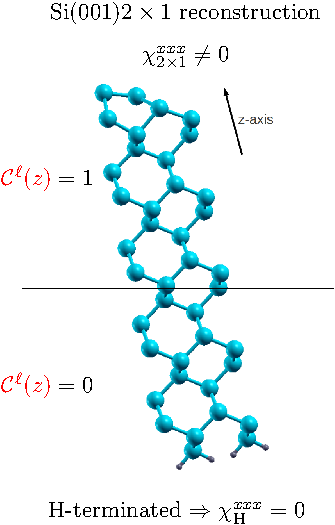
\includegraphics[scale=.8]{images/si2x1-crop}
\caption{(color on line) The slab shows a front clean Si(001)$2\times 1$ surface,
  while the back surface is ideally terminated Si bulk, where the  
  dangling bonds are H (small balls) saturated. This picture shows 12  
  Si atomic layers and one H atomic layer. 
\label{si2x1}} 
\end{figure} 
The idea for such an slab is that the cristalline symmetry of the
H terminated surface imposes that $\chi_{\mathrm{H}}^{xxx}=0$, while
for the $2\times 1$ surface there is not such symmetry restriction and
then, $\chi_{2\times 1}^{xxx}\ne 0$.
Therefore, due to this fact, calculating $\chi^{xxx}$ for the full-slab
or the half-salb that contains the $2\times 1$ surface,\cite{nota1}
 ought to give the same result, since the contribution from the H
 saturated  surface is zero any way. Then, for this slab one must check
 whether or not this relation is satisfied,
\begin{align}\label{hs}
\chi_{\mathrm{half-slab}}^{xxx}(-2\go;\go,\go) 
=
\chi_{\mathrm{full-slab}}^{xxx}(-2\go;\go,\go)
,
\end{align}
where
$\chi_{\mathrm{half-slab}}^{xxx}(-2\go;\go,\go)$ is calculated using
$C^\ell(z)=1$ un the upper half of the salb, that contains the
$2\times 1$ surface reconstruction, as seen in
Fig.~\ref{si2x1},
whereas $\chi_{\mathrm{full-slab}}^{xxx}(-2\go;\go,\go)$ is calculated using
$C^\ell(z)=1$ through the full slab.
Indeed, in what follows we show the results of such a comparison.

The self-consistent ground state and their Kohn-Sham states were
calculated in the frame-work of DFT-LDA,
with the use of the plane-wave ABINIT
code.\cite{abinit}
We used
Troullier-Martins
pseudopotentials,\cite{troullierPRB91} 
that are 
fully separable nonlocal pseudopotentials in the 
Kleinman-Bylander 
form;\cite{kleinmanPRL82}
the contribution of $\bfv^\nl$ to Eq.~\eqref{chis},
can be calculated, as explained in Appendix \ref{vesnl}; 
we use the DP code for this end.\cite{francesco}
The $2\times 1$ and the H surfaces are relaxed \textcolor{red}{Nicolas 
  some details}, where we find agreement with previous results for 
both surfaces.\cite{relax} For instance the Si-H bond distance is 1.48 
$\AA$ ??. The unit cell has two atoms, making the calculation
computational very heavy. The vacuum size is equivalent to one quarter
of the
size of the slab, thus avoiding spurious effects from the possible
tunneling of the wave function of the contiguous surfaces of the full
crystal formed by the repeated super cell scheme.\cite{mendozaPRB06}    

Spin-orbit effects, local field effects, and the consequences of the
electron-hole
attraction\cite{leitsmannPRB05,trollePRB14} on the SHG process are neglected. 
Although all these effects are important for the optical response of a
semiconductor, 
their calculation is still an open question and a numerical challenge
that ought to be pursued. 
However this endeavor is beyond the scope of this paper. 
For a given size  
of the slab,  we find converged spectra
for all the quantities of interest in this
work, 
and the most important parameters are
an energy cut-off of 10 Ha,
a number 
of conduction bands equal to the number of valence 
bands,
and a set of 244 $\bfk$-points
is used for
the linear analytic tetrahedron method used in the evaluation
the Brillouin zone integrals for of Eq.~\eqref{chis}, where special care
was taken to examine the double resonances.\cite{nastosPRB05}
Double resonances occur if for a given frequency $\omega$
there can be resonant
transitions at both frequencies $\omega$ and 2$\omega$,
 that is, if there is a
region in the Brillouin zone such that
$\omega_{cv}(\bfk)=2 \omega_{c'v}(\bfk)$
For these $\bfk$ points the perturbation theory used to calculate
the spectrum breaks down, since there is real population excited,
which in a correct calculation must be taken into account. These
points introduce sharp spikes in the spectrum that can, in
principle, affect the low-frequency results, since the response at
frequencies below the band gap is computed from the Kramers-Kronig
relation. However, in agreement with Ref.~\onlinecite{nastosPRB05}
 we find here
that the double resonances affect the low-frequency results by less
than 2\%. 
Finally, all the spectra are calculated with an energy Gaussian smearing of  0.15 eV {\color{red}Chon??} 
\begin{figure}
\centering 
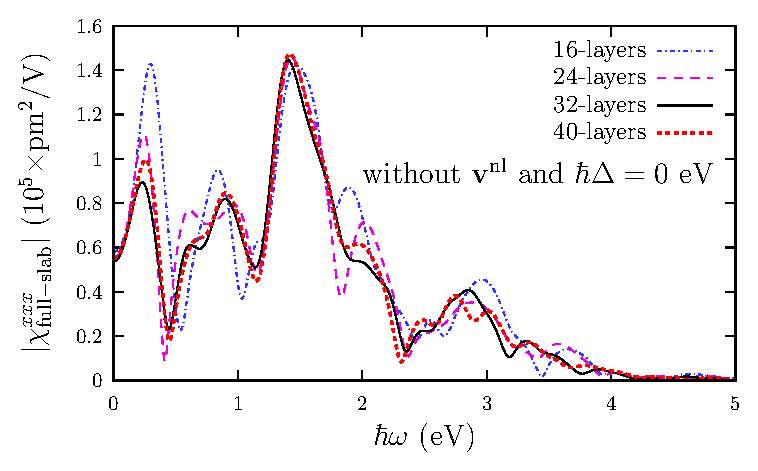
\includegraphics[scale=.8]{plots/fig1}
\caption{(color on line) 
$|\chi_{\mathrm{half-slab}}^{xxx}|$ vs $\hbar\omega$ for different slabs with 16, 24, 32 
and 40 atomic Si layers. The fron surface of the slab presents a 
$2\times 1$ reconstruction, whereas the back sufrace is ideally bulk 
terminated where the dangling bonds are H-saturated. 
\label{fig1}} 
\end{figure}
\begin{figure}
\centering 
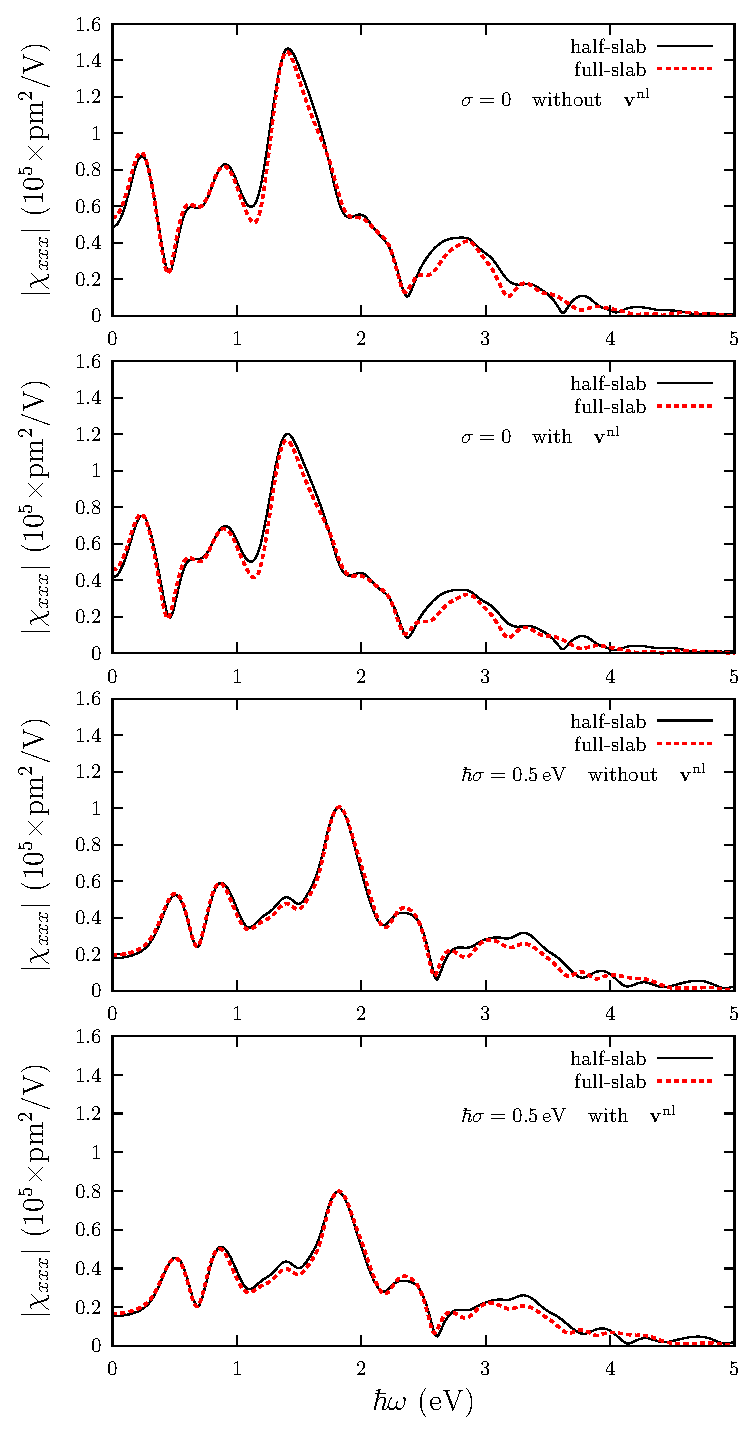
\includegraphics[scale=.8]{plots/fig2}
\caption{(color on line) 
$\chi^{xxx}_{\mathrm{half-slab}}$
and 
$\chi^{xxx}_{\mathrm{full-slab}}$
vs $\hbar\omega$ for a slab of 32 
atomic Si layers plus one layer of H. 
\label{fig2}} 
\end{figure}

To obtain Eqs.~\eqref{tau.1}  and \eqref{tau.1n}, required in
Eq.~\eqref{chis},
we see that the
evaluation of the commutator $[\bfr,\bfv^\nl]$ is required as it is
outlined in Appendix \ref{appvnl}; second order derivatives
are required to do such evaluation, making the numerical
procedure very
time consuming. Indeed this time is much higher than the already
lengthy time needed for the calculation of the contribution of
$\bfv^\nl$, proportional to only first order derivatives, as seen in
Appendix \ref{vesnl}. 
On top of this, the memory required is also very demanding for both
$\bfv^\nl$ and $[\bfr,\bfv^\nl]$.
However, the contribution coming from 
$[\bfr,\bfv^\nl]$, turns out to be very small,\cite{valerie} and
therefore we neglect it in this work.

In Fig.~\ref{fig1} we show $|\chi_{\mathrm{half-slab}}^{xxx}|$
 for a
slab of 16, 24, 32, and 40 Si atomic layers. We see that 
$|\chi_{\mathrm{half-slab}}^{xxx}|$ for
16 and 24
layers are different from each other, and different from that of 32
and 40 layers,
that are very similar to each other.
As explained above,
the calculation of the contribution given by
$\bfv^\nl$ is computational very demanding. A good
compromise between the accuracy in the convergence of
$\chi^{xxx}_{\mathrm{half-slab}}$,
 as a function of the number
of atomic layers in the slab, and the computational burden, is to take
the slab with 32 Si atomic layers, as representative of our system
in question.
In Fig.~\ref{fig2}
we compare 
$\chi^{xxx}_{\mathrm{half-slab}}$  
vs. 
$\chi^{xxx}_{\mathrm{full-slab}}$, 
for the four different possibilities of including or not including the
effects of $\bfv^\nl$ and having or not having a scissors correction
$\hbar\sigma$.
We see that for all four instances the comparison between
$\chi^{xxx}_{\mathrm{half-slab}}$ 
and
$\chi^{xxx}_{\mathrm{full-slab}}$,
is very good. Indeed, where the value of $|\chi^{xxx}|$ is large the
difference is very small, and when its value is small, the difference
are just slightly larger, but the spectra is so close to zero that the
differences are not very meaning full; this diferences would become
smaller as the number of atomic layers is increased. However, with 32
layers is more than enough to 
confirm that the extraction of the surface second
harmonic susceptibility from the $2\times 1$ surface is 
readily possible using the formalism contained in Eq.~\eqref{chis}.

Although in a forthcoming publication we will present a study of SSHG
from several Si surfaces where experimental results are available, we
proceed to explain, without confronting with experiment ({\color{red}
Nicolas are there any for this particular component?}), some of the
features seen in 
$|\chi^{xxx}_{2\times 1}|$,  
that is of coures given by
$|\chi^{xxx}_{\mathrm{half-slab}}|$.
First of all, from Fig.~\ref{fig2} 
we see a series of resonances 
that come from the 1$\omega$ and 2$\omega$ terms in
Eq.~\eqref{chis}. The 2$\omega$ resonances naively would start below
$E_g/2$ where $E_g=3.4$ eV is
the band gap of bulk Si. However we see that there are several
resonances well below 1.7 eV, and of course, these resonances are
coming from the electronic states of the $2\times 1$ surface, that lie
inside the gap, that are the well known surface states.
We see that the effect of $\bfv^\nl$ reduces the value of   
$|\chi^{xxx}_{2\times 1}|$,\cite{note2}  
without changing the form of the spectra, as can be confirmed from
both cases of zero and non-zero scissors correction.
Also, we see that the scissors correction shifts the spectra to higher
energies, as expected, however, contrary to the case of linear optics,\cite{cabellosPRB09}
the shifting is not rigid. This is because, the second harmonic optical
response mixes 1$\omega$ and 2$\omega$ transitions, as can be seen from
Eq.~\eqref{chis}, and thus the spectra is not rigidly shifted. 
\begin{figure}
\centering 
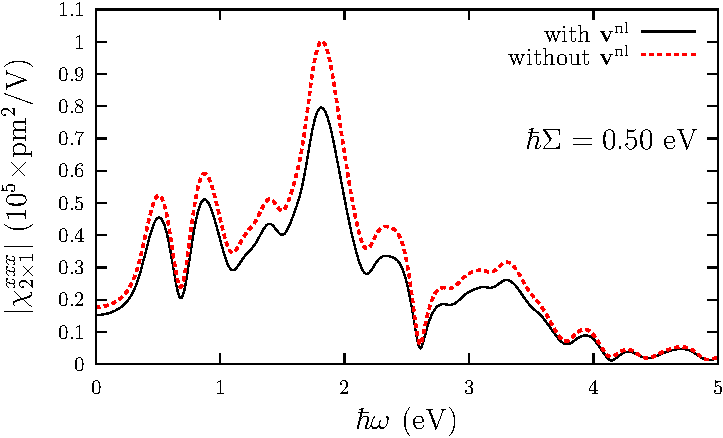
\includegraphics[scale=.8]{plots/fig3}
\caption{(color on line) 
$\chi^{xxx}_{2\times 1}$
vs $\hbar\omega$ for a slab of 32 
atomic Si layers plus one layer of H, for two different values of 
the scissors correction $\hbar\sigma$.
\label{fig3}} 
\end{figure}

Finally, in Fig.~\ref{fig3} we compare 
$|\chi^{xxx}_{2\times 1}|$ for two values of $\hbar\sigma$. Indeed,
the value of $\hbar\sigma=0.5$ eV, used above, is the ``average'' GW gap taken from 
Refs.~\onlinecite{rholfingPRB95} which is in agreement with \onlinecite{garciaCPC01}, and  
the value of $\hbar\sigma=0.63$ eV is the ``average'' GW gap taken from 
Refs.~\onlinecite{asahiPRB00}, where more $\bfk$ points in the
Brillouin zone were used.
We see that the fist two peaks are almost rigidly shifted with a small
difference in height, while the rest of the peaks are modified
substantially. This behavior, comes from the fact that the first two
peaks are almost related to the 1$\omega$ resonances of
Eq.~\eqref{chis}, and the other peaks are a combination of 1$\omega$
and 2$\omega$ resonances, thus giving a more different spectrum. This
way we see that small changes in the value of the scissors shift can affect the
$|\chi^{xxx}_{2\times 1}|$ quite dramatically.


%%%%%%%%%%%%%
\appendix 
\section{}\label{appe}
We give explicit expressions for the quantities used in the evaluation 
of Eq.~\eqref{chis}; when appropriate, some 
intermediate steps are given for their derivation. 
%%%%
\subsection{ Expressions for 
\texorpdfstring{${\cal V}^{\ell,a}_{nm}(\bfk)$, 
${\cal C}^{\ell}_{nm}(\bfk)$ 
and
$({\cal C}^{\ell}_{nm}(\bfk))_{;\bfk}$
}{Vnm and Cnm}}\label{calpcalc}

Expanding the wave function in plane waves we obtain
\begin{align}\label{eni.1}
\psi_{n\bfk}(\bfr)=\sum_\bfG A_{n\bfk}(\bfG)e^{i(\bfk+\bfG)\cdot\bfr}
,
\end{align}
where $\{\bfG\}$ are the reciprocal basis vectors satisfying
$e^{\bfR\cdot\bfG}=1$, with $\{\bfR\}$ the translation vectors in real
space, and $A_{n\bfk}(\bfG)$ {\color{\chon} the} expansion coefficients. Using
$m_e\bfv=-i\hbar\bfgnabla$ into 
Eq.~\eqref{vcali}
we obtain,\cite{mendozaPRB06}
\begin{align}\label{eni.2}
\calbv^\ell_{nm}(\bfk)=
\frac{\hbar}{2m_e}
\sum_{\bfG,\bfG'} A^*_{n\bfk}(\bfG')  A_{m\bfk}(\bfG)
(2\bfk+\bfG+\bfG')
\gd_{\bfG_\parallel \bfG'_\parallel}  
f^\ell(G_\perp-G'_\perp)
,
\end{align}   
where
\begin{align}\label{vnl.9}
f^\ell(g)=\frac{1}{L}\int_{z_\ell-\gD^b_\ell}^{z_\ell+\gD^f_\ell} e^{igz}dz  
 ,
\end{align}
with $f^{\ell*}(g)=f^\ell(-g)$. 
{\color{\chon} The} reciprocal lattice vectors $\bfG$ are 
decomposed into components
{\color{\chon} parallel ($\bfG_\parallel$), and perpendicular ($G_\perp \hat z$)} 
to the surface, so
that $\bfG = \bfG_\parallel + G_\perp\hat z$.
The double summation over the $\bfG$ vectors can be 
{\color{\chon} calculated efficiently} by  
creating a pointer array to identify all the plane-wave coefficients  
associated with the same $G_\parallel$.  
Likewise we obtain that
\begin{align}\label{eni.4}
\calc^\ell_{nm}(\bfk)=
\sum_{\bfG,\bfG'} A^*_{n\bfk}(\bfG')  A_{m\bfk}(\bfG)
\gd_{\bfG_\parallel \bfG'_\parallel} 
f^\ell(G_\perp-G'_\perp)
.
\end{align}  
If $\calc^\ell(z)=1$, {\color{\chon} then $f^\ell(g)=\gd_{g0}$ and we 
obtain the full-slab/bulk values, 
$\bfv_{nm}(\bfk)$ and $\calc^\ell_{nm}(\bfk)=\gd_{nm}$,
from Eqs.~\eqref{eni.2} and \eqref{eni.4}}.

We use Eqs.~\eqref{rnminn}, \eqref{conmri3n}, and \eqref{gendevnn},
along with $[\bfr,F(\bfr)]=0$, valid for 
and any function $F(\bfr)$, 
{\color{\chon} to }obtain
\begin{align} 
(\calc^\ell_{nm})_{;\bfk}
&=
i
\sum_{q} 
 \left(\bfr_{nq}
\calc^\ell_{qm}
-
\calc^\ell_{nq}
\bfr_{qm}
\right) 
+i\bfr_{nm}(\calc^\ell_{mm}-\calc^\ell_{nn}) 
,
\end{align} 
where we remind the reader that $\bfr_{nm}$ 
{\color{\chon} is} calculated through
Eq.~\eqref{chon.10} for LDA. 

%%%%
\subsection{Expressions for 
\texorpdfstring{$(\calv^{\ell,\lda,a}_{nm})_{;k^b}$}{Vnonlocal}
and \texorpdfstring{$(r^a_{nm})_{;k^b}$}{Vnonlocal}
for non-local potentials}\label{appvnl}

Using Eqs.~\eqref{rnminn}, \eqref{conmri3n}, \eqref{gendevnn}, and
defining 
$
\calt^{\rma\rmb}\equiv[r^{\rmb},\calv^{\lda,\rma}]
\equiv
[r^{\rmb},\calv^\rma]
$
one can show that{\color{\chon} 
\begin{align}\label{nmesn}
(\calv^{\ell,\lda,\rma}_{nm})_{;k^{\rmb}}&=
\calt_{nm}^{\ell,\rma\rmb}
+i
\sum_{q}
\bigg(
r^{\rmb}_{nq}  
\calv^{\ell,\lda,\rma}_{q m}
-
\calv^{\ell,\lda,\rma}_{nq}   
r^{\rmb}_{q m}
\bigg)  
+i  
r^{\rmb}_{nm}
\Delta^{\ell,\rma}_{mn}
,
\end{align}}
where
\begin{eqnarray}\label{tdel}
\Delta^{\ell,\rma}_{mn}
=
\calv^{\ell,\lda,\rma}_{nn}  
-
\calv^{\ell,\lda,\rma}_{mm}  
,
\end{eqnarray} 
and
\begin{align}\label{tau.1}
\calt_{nm}^{\ell,\rma\rmb}
=
\frac{\hbar}{m_e}\gd_{\rma\rmb}
C^\ell_{nm} 
-i 
\sum_q 
[r^{\rmb},v^{\nl,\rma}]_{nq}C^\ell_{qm} 
.
\end{align}  
The matrix elements $[r^{\rmb},v^{\nl,\rma}]_{nm}$
are calculated in Appendix \ref{calt}.
% is small
%compared to the other terms, thus we neglect it throwout this work.\cite{valerie} 
Notice that
{\color{\chon} 
$(v^{\lda,\rma}_{nm})_{;k^{\rmb}}$} is obtained 
from Eq.~\eqref{nmesn} by 
taking 
{\color{\chon} $C^\ell(z)=1$ or $C^\ell_{nm}=\gd_{nm}$.}

To obtain $(r^{\rma}_{nm})_{;k^{\rmb}}$ we use Eq.~\eqref{chon.10} to
write
$(r^{\rma}_{nm})_{;k^{\rmb}}
=(v^{\lda,\rma}_{nm}/i\go^\lda_{nm})_{;k^{\rmb}}
$ {\color{\chon} and} simply apply the chain rule,
\begin{align}\label{rka}
(r^{\rma}_{nm})_{;k^{\rmb}}
&=
t^{\rma\rmb}_{nm}
+
\frac{ 
r^{\rmb}_{nm}
\Delta^{\rma}_{mn}
+r^{\rma}_{nm}
\Delta^{\rmb}_{mn}
}
{\go^\lda_{nm}}
+
\frac{i}{\go^\lda_{nm}}
\sum_{q}
\bigg(
\go^\lda_{q m} 
r^{\rmb}_{nq} 
r^{\rma}_{q m}
-
\go^\lda_{nq} 
r^{\rma}_{nq} 
r^{\rmb}_{q m}
\bigg)
,
\end{align} 
where 
\begin{eqnarray}\label{del}
\Delta^{\rma}_{mn}
=
v^{\lda,\rma}_{nn}  
-
v^{\lda,\rma}_{mm}  
,
\end{eqnarray}
and{\color{\chon} 
\begin{align}\label{tau.1n} 
t_{nm}^{\rma\rmb}
=\frac{\hbar}{m_e}\gd_{ab}\gd_{nm} 
-i [r^{\rmb},v^{\nl,\rma}]_{nm} 
.
\end{align}}
Eq.~\eqref{rka} generalizes the usual expresion of
$(r^a_{nm})_{;k^b}$ for {\color{\chon} a} local 
{\color{\chon} Hamiltonian}
\cite{aversaPRB95,nastosPRB05,cabellosPRB09,rashkeevPRB98}
to
the case of a
nonlocal Hamiltonian.
Note that the layered term
$\calt^{\ell,\rma\rmb}_{nm}$ reduces to $t^{\rma\rmb}_{nm}$
{\color{\chon} for the full-slab/bulk case.}

%%%%
\subsection{Matrix elements of 
\texorpdfstring{$\calbv^{\ell,\nl}$}{Vnonlocal},
\texorpdfstring{$\bfv^\nl$}{Vnonlocal}, and 
\texorpdfstring{$[\bfr,\bfv^\nl]$}{[r,vnl]}}
\label{vesnl}

We take Eq.~\eqref{vcali}
and use
$\sum_{\bfG}\ket{\bfk+\bfG}\bra{\bfk+\bfG}=1$, 
with
$\braket{\bfr}{\bfk+\bfG}=(1/\sqrt{\gO})
\mathrm{exp}(i(\bfk+\bfG)\cdot\bfr)$
{\color{\chon} to} obtain,\cite{mottaCMS10}
\begin{align}\label{vnl.5}
\calbv^{\ell,\nl}_{nm}(\bfk)&=\frac{1}{2}
\sum_{\bfG}
\Big(
\bra{n\bfk} C^\ell(z) 
\ket{\bfk+\bfG}\bra{\bfk+\bfG}
\bfv^\nl \ket{m\bfk}
+
\bra{n\bfk}
\bfv^\nl  
\ket{\bfk+\bfG}\bra{\bfk+\bfG}
C^\ell(z) \ket{m\bfk}
\Big)
\nonumber\\
&=\frac{1}{2 \hbar}
\sum_{\bfG}
\left(
\calf^{\ell*}_{n\bfk}(\bfG) 
\calh_{m\bfk}(\bfG) 
+
\calh^*_{n\bfk}(\bfG) 
\calf^\ell_{m\bfk}(\bfG) 
\right) 
,
\end{align}  
where 
we have defined  
\begin{align}\label{vnl.10}
\calf^\ell_{n\bfk}(\bfG) 
=
\sum_{\bfG'} 
A_{n\bfk}(\bfG') 
\gd_{\bfG_\parallel \bfG'_\parallel}f^\ell(\bfG'_\perp-\bfG_\perp) 
,
\end{align} 
\begin{align}\label{vnl.11}
\calh_{n\bfk}(\bfG)&=
\sum_{\bfG'} 
A_{n\bfk}(\bfG') 
(\nabla_{\bfK}+\nabla_{\bfK'})  
V^\nl(\bfK,\bfK') 
,
\end{align}
and $\bfK=\bfk+\bfG$, $\bfK'=\bfk+\bfG'$.
For fully  separable pseudopotentials in the   
Kleinman-Bylander (KB) form,\cite{mottaCMS10,kleinmanPRL82,adolphPRB96}  
the  
matrix elements 
 $\bra{\bfK}  
V^\nl  
\ket{\bfK'}
=V^\nl(\bfK,\bfK')  
$ 
{\color{\chon} and} their $\bfK$ and $\bfK'$ gradient 
can be readily calculated.\cite{mottaCMS10,adolphPRB96,gordienkoRPJ04,fuchsCPC99} 
We have 
implemented 
the calculation of $\calbv^{\ell,\nl}_{nm}(\bfk)$ with the help {\color{\chon} of} 
the \depe~code.\cite{francesco}
{\color{\chon} We obtain $\bfv^{\nl}_{nm}(\bfk)$ from the previous three 
expressions by t}aking $C^\ell(z)=1$, which implies 
{\color{\chon} that} $f^\ell(g)=\gd_{g0}$.

%%%%
%\subsection{Matrix elements of $[\bfr,\bfv^\nl]$}\label{calt}
\label{calt}
Using Eq.~\eqref{vnl} we define
\begin{align}\label{3.1}
\call^{\rma\rmb}_{nm}(\bfk) 
\equiv\frac{1}{i\hbar}
\bra{n\bfk}
[ r^{\rma}, v^{\nl,\rmb}]
\ket{m\bfk}
=
\frac{1}{\hbar^2}
\bra{n\bfk}
\big[ r^{\rma},[ V^\nl, r^\rmb]\big]
\ket{m\bfk}
,
\end{align} 
{\color{\chon} and we expand the triple commutator,}
\begin{align}\label{3.5}
\call^{\rma\rmb}_{nm}(\bfk) 
&=
\frac{1}{\hbar^2\gO}
\sum_{\bfG,\bfG'} 
A^*_{n\bfk}(\bfK) 
A_{m\bfk}(\bfK')
\int
d\bfr d\bfr'
 e^{-i\bfK\cdot\bfr}
\Big(
r^{\rma}
V^\nl(\bfr,\bfr')
r'^\rmb
-
V^\nl(\bfr,\bfr')
r'^\rma
r'^{\rmb}
\nonumber\\
&-
r^\rmb
r^{\rma}
V^\nl(\bfr,\bfr')
+
 r^\rmb
V^\nl(\bfr,\bfr')
r'^{\rma}
\Big) 
 e^{i\bfK'\cdot\bfr'}
,
\end{align} 
where 
$V^\nl(\bfr,\bfr') = \bra{\bfr} V^\nl\ket{\bfr'}$.
We use the following identity
\begin{align}\label{3.4}
&
\Big(
\frac{\partial^2}{\partial K^\rma\partial K'^\rmb}
+
\frac{\partial^2}{\partial K'^\rma\partial K'^\rmb}
+
\frac{\partial^2}{\partial K^\rma\partial K^\rmb}
+
\frac{\partial^2}{\partial K^\rmb\partial K'^\rma}
\Big)
\int 
d\bfr d\bfr' 
 e^{-i\bfK\cdot\bfr}
V^\nl(\bfr,\bfr') 
e^{i\bfK'\cdot\bfr'}
\nonumber\\
&=
\int d\bfr d\bfr'
 e^{-i\bfK\cdot\bfr}
\Big( 
r^{\rma} 
V^\nl(\bfr,\bfr') 
r'^\rmb
- 
V^\nl(\bfr,\bfr') 
r'^\rma 
r'^{\rmb}
- 
r^\rmb 
r^{\rma} 
V^\nl(\bfr,\bfr')
+
 r^\rmb 
V^\nl(\bfr,\bfr') 
r'^{\rma}
\Big)  
e^{i\bfK'\cdot\bfr'}
,
\end{align}
to write
\begin{align}\label{3.7}
\call^{\rma\rmb}_{nm}(\bfk)
&=
\frac{1}{\hbar^2\gO}
\sum_{\bfG,\bfG'} 
A^*_{n\bfk}(\bfK) 
A_{m\bfk}(\bfK')
\Big(
\frac{\partial^2}{\partial K^\rma\partial K'^\rmb}
+
\frac{\partial^2}{\partial K'^\rma\partial K'^\rmb}
+
\frac{\partial^2}{\partial K^\rma\partial K^\rmb}
+
\frac{\partial^2}{\partial K^\rmb\partial K'^\rma}
\Big)
\bra{\bfK} 
V^\nl 
\ket{\bfK'}, 
\nonumber\\
\end{align} 
where
\begin{align}\label{vkk}
\bra{\bfK} 
V^\nl 
\ket{\bfK'} 
=
\int 
d\bfr d\bfr' 
 e^{-i\bfK\cdot\bfr}
V^\nl(\bfr,\bfr') 
e^{i\bfK'\cdot\bfr'}
,
\end{align}
The double derivatives with respect to $\bfK$ and $\bfK'$ 
can be worked out explicitly {\color{\chon} and} 
${\cal L}^{\rma\rmb}_{nm}(\bfk)$
{\color{\chon} can} be finally calculated.\cite{valerie}

%%%%
\subsection{Expressions for  \texorpdfstring{$\bfv^{\ell,S}_{nm}$}{Vnm}
and
\texorpdfstring{$\Big({\calbv}^{\ell,S}_{nm}\Big)_{;\bfk}$}{(Vnm);kb}
}\label{calvs} 

From Eq.~\eqref{vcali}
\begin{align}\label{a.3b}
\calbv^{\ell,S}_{nm}
&=
\frac{1}{2}\sum_q\left(   
\bfv^S_{nq}\calc^\ell_{qm}+\calc^\ell_{nq}\bfv^S_{qm}
\right)  
,
\end{align}    
where $\sum_q\ket{q\bfk}\bra{q\bfk}=1$ was used
{\color{\chon} and $\bfv^S_{nm}$ is} given in Eq.~\eqref{chon.2}.
Taking the generalized derivative of Eq.~\eqref{a.3b}
{\color{\chon} and} applying
the chain rule, we obtain
\begin{align}\label{a.3bn}
\left(\calbv^{\ell,S}_{nm}\right)_{;\bfk}
&=
\frac{1}{2}\sum_q\left(
(\bfv^S_{nq})_{;\bfk}\calc^\ell_{qm}
+    
\bfv^S_{nq}(\calc^\ell_{qm})_{;\bfk}
+
(\calc^\ell_{nq})_{;\bfk} \bfv^S_{qm}
+
\calc^\ell_{nq} (\bfv^S_{qm})_{;\bfk}
\right)  
,
\end{align}    
{\color{\chon} and considering} 
Eq.~\eqref{chon.2}, 
\begin{align}\label{choni.1}
(\bfv^S_{nm})_{;\bfk}=i\gs f_{mn}
(\bfr_{nm})_{;\bfk}
,
\end{align}
{\color{\chon} is in total} 
agreement with Eq. A(6) of Ref.~\onlinecite{cabellosPRB09}.

%%%%%%%%%%%%%%
\bibliography{ref}% 
\end{document}  %
%%%%%%%%%%%%%%


\section{Introduction}\label{intro}

Second harmonic generation (SHG) is a powerful spectroscopic tool for 
studying the optical properties of surfaces and interfaces since it has 
the advantage of being surface sensitive. Within the dipole approximation, 
inversion symmetry forbids SHG from the bulk of controsymmetric materials. 
SHG is allowed at the surface of these materials where the inversion symmetry 
is broken and should necessarily come from the localized surface region. 
SHG allows the study of the structural atomic arrangement and phase 
transitions of clean and adsorbate covered surfaces. Since it is also an 
optical probe it can be used out of UHV conditions and is non-invasive 
and non-destructive. Experimentally, new tunable high intensity laser systems 
have made SHG spectroscopy readily accessible and applicable to a wide range 
of systems.\cite{downer_optical_2001,lupke_characterization_1999}

However, theoretical development of the field is still an ongoing 
subject of research. Some recent advances for the cases of semiconducting 
and metallic systems have appeared in the literature, where the use of 
theoretical models with experimental results have yielded correct 
physical interpretations for observed SHG spectra.
\cite{
downer_optical_2001,
mendozaPRB01,
lim_optical_2000,
gavrilenko_optical_2000,
mendozaPRB99,
mendozaPRL98,
mendozaPRB96,
mendozaPRB97,
guyotPRB90} 

In a previous article\cite{mendoza_epioptics_2001} we reviewed some 
of the recent results in the study of SHG using the velocity gauge 
for the coupling between the electromagnetic field and the electron. 
In particular, we demonstrated a method to systematically analyze the 
different contributions to the observed SHG peaks.\cite{arzatePRB01} 
This approach consists of separating the different contributions to 
the nonlinear susceptibility according to 1$\omega$ and 2$\omega$ 
transitions, and the surface or bulk nature of the states among 
which the transitions take place. 

To compliment those results, in this article we review the calculation 
of the nonlinear susceptibility using the longitudinal gauge. We show 
that it is posible to clearly obtain the ``layer-by-layer'' contribution 
for a slab scheme used for surface calculations.




